\documentclass[12pt,%
               draft,%
               a4paper]{uiothesis}

\usepackage[T1]{fontenc}
\usepackage[utf8x]{inputenc}
\usepackage{graphicx}
\usepackage{longtable}
\usepackage{lscape}
\usepackage{natbib}
\usepackage{paralist}
\usepackage{ragged2e}

\title{Social Navigation on the Social Web}
\subtitle{Unintrusive Prototyping in Established Spaces}
\author{Eivind Uggedal}

%\includeonly{%
%acknowledgements,%
%introduction,%
%background,%
%methodology,%
%analysis,%
%implementation,%
%selection.of.third.party.software,%
%discussion,%
%conclusion,%
%content.inventory,%
%questionnaire,%
%source.code,%
%}

\begin{document}
  \chapterstyle{uio}
  \pagestyle{uio}
  \maxsecnumdepth{subsubsection}

  \frontmatter
    \pagenumbering{alph}
    \maketitle
    \pagenumbering{roman}
    \clearpage
    \tableofcontents
    \clearpage
    \listoffigures
    \clearpage
    \listoftables
    \clearpage
    \listofsourcecode
    \chapter{Acknowledgements}
I would like to thank
Andreas Dieberger,
Peter Brusilovsky, and
Robert Mertens
for allowing me to freely use illustrations from
some of their published articles.


  \mainmatter
    \chapter{Introduction}

% The point of the introduction is to answer: what is this thesis about?
% Explain this in four steps by:
%
%   * Why you have chosen this topic rather than any other. Examples:
%       - has been neglected
%       - much discussed but not properly and fully
%   * Why this topic interests you.
%   * The kind of research approach or academic disciple you will utilize.
%   * Your research questions or problems.
%
% The role of the introduction, like the abstract, is to orient your readers.
% This is best done clearly and succinctly.

The web is becoming increasingly more social as
``the digital domain has seen a significant growth in the scale and richness
of on-line communities'' \citep[p.~44]{backstrom06}.
\citet[ch.~1, p.~2]{rosa07} reports that the
use of blogs in the general public%
\sidenote{%
  Represented with a total of 6,545 respondents
  to a survey conducted in Canada, France, Germany, Japan,
  the United Kingdom, and the United States.
}
have grown significantly the last 18 months as can be seen in
Table~\ref{table:blog.usage}
(p.~\pageref{table:blog.usage}).
More than one third of these blog users have contributed actively
by writing blog articles\citep[ch.~1, p.~6]{rosa07}.
It has been argued that web citizens'
familiarity with blogging laid the groundwork for the explosion we are seeing
in user participation in web communities \citep[ch.~2.2]{beer07}.

\sidetable{Blog Usage}{%
  \label{table:blog.usage}
  \begin{tabular}{lll}

    \toprule
    Year & Passive & Active \\
    \midrule

    2005 & 16\% & n/a \\
    2007 & 45\% & 17\% \\

  \end{tabular}
}

At the same time technological
advances and maturity have made it easy and cheap to create new communities.
This means that we're seeing an abundance of such communities appear.
They're all competing to establish self sufficient user bases, and if the
objective is to achieve large profits, to adopt as many users
as possible. This creates a strong incentive to come up with interesting new
features and best your competitors when it comes to pleasing your users.
As a result we're seeing rapid innovation in this area of the web infamously
coined ``Web 2.0''.%
\sidenote{%
  Web 2.0 was first used as the name of a conference arranged by
  O'Reilly Media. The ``2.0'' part of the conference name was then used to
  signify the revival of interest in the web after the dot-com bubble in the
  early 21st century \citep{oreilly07}.
  Later the founder of O'Reilly Media, Tim O'Reilly, defined
  the term as the characteristics of the web services that survived the dot-com
  bubble and the web services he deemed to be the best newcomers to the
  field \citep{oreilly05}.
}

This thesis focuses on navigational problems and only those which are of a
social nature. Having efficient and easy to use navigation is clearly
essential for serving your users' interests. As the content on the web to a
higher degree than before are user generated it has become almost impossible
for the creators of a given web service to design sound navigation without
relying on their loyal users. Instead such structures have to be organically
grown by designing navigational schemes that harness the work your user base
is conducting as they use your service. This is the essence of social
navigation as the first definition of the term clearly and succinctly
captures:

\begin{quote}
In social navigation, movement from one item to another is provoked as an
artifact of the activity of another or a group of others. \citep{dourish94} 
\end{quote}

\section{Motivation}

Social navigation are as we've seen a well defined term within the academic
community and there have been a handful of studies on it's applicability in
context of the web \citep{dieberger97,wexelblat99}. % more studies needed
Most of this research took place in the early days of the
web---preceding our current area of Web 2.0.
As \citet{beer07} notes: ``\ldots `internet time' now runs at at a clock speed
several orders of magnitude faster than that of academic research''.
We described earlier the
growth we're seeing of web services with social aspects and
we firmly believe that these are bound to provide
for innovations in the space of navigation. It would therefore be interesting
to look at some of the state-of-the-art social web services and look at what
contributions they have made to the field of social navigation.

We are currently lacking information on how one can use social navigation
consciously in a web application design process. Such navigational schemes
seem to be created without guidance and many times as an afterthought.
It appears that methods for establishing incentives for user participation
is the focal point of web architecture design today. Even though such
approaches can result in sound and interesting navigation it's our impression
that a focus on solving users' navigational problems is more beneficial for
the usability of a web service.

\section{Objective}

By collecting examples of good navigational implementations in the wild,
analyzing them, and categorize them we hope to offer a structured view of the
field of social navigation. We offer this information in the way of a taxonomy
of useful social navigation techniques.
As we are unaware of any established technique for
conducting such a study on real world navigation systems we create our own
method as we go---fine tuning it as we learn from our experiences.

We try to improve an existing web service by using some of the techniques
established in our initial research of how social navigation is leveraged
in real world applications. More specifically we are prototyping possible
navigational improvements for the Norwegian Broadcasting Corporation's joint
TV, radio, and Internet project: \emph{Ur\o{}rt}---a service where artists upload
their demos and get valuable playtime on radio and TV if their products are
judged to be of sufficient quality. Our focus is on the projects
web community\sidenote{Available at \url{http://nrk.no/urort}} where users can
interact in a social manner in addition to uploading their songs.

Going in and making changes to an existing web service can be both an
daunting and time consuming task. First one have to establish a trustworthy
relationship with the creators of such a service so that they are certain
you're not introducing bugs in their production software. Secondly, grasping the
code base, third party libraries, and development tools of such a software
project demands a lot of upfront effort before any real development work can
begin. This goes against the prototypical process we intended to use while
experimenting with Ur\o{}rt.

Even though we've had an ongoing dialog with the developers of Ur\o{}rt we
decided to create our prototype as a layer on top of their service. By using a
extension\sidenote{Specifically Greasemonkey, an extension allowing for
customization of presentation and behavior of web pages. Available at
\url{http://www.greasespot.net}} for the open source Firefox%
\sidenote{Available at \url{http://firefox.com}}
web browser we were able to make changes and additions to the way Ur\o{}rt were
presented to users who were participating in our study. We were able to create
a back end for the additional data and behavior our new functionality required
with the frameworks and programming language we found to be most efficient in
a prototypical process. This resulted in a transparent experience for our end
users as long as they had taken the necessary steps to set up the browser
extension and our script.

With our technical solution in place we were able to test how it performed in
practice by conducting ``some sort of user observation'' (not decided) and
(possibly) more quantitative surveys.

This leads to the research question we had in mind while conducting
the tasks described above:

\begin{quote}
  How can social navigation influence usage of established web services?
\end{quote}

The role of this question have been to give our research direction, show where
it's boundaries were, keep us focused, and point to the needed methods and
data \citep[p.~77]{silverman05}.

% hypotheses ?

\section{Contributions}

Contributions from our research on social navigation is threefold:

\begin{description}
  \item[Informing navigational design] by giving a structured overview of
    various navigational schemes in use today.
  \item[Transparent prototyping techniques] by sharing experiences from
    creating a unobtrusive shell of navigational designs on top of an
    existing web service.
  \item[Applicability of social navigation] by showing results from real
    users' usage of social navigation designs.
\end{description}

\section{Outline}

Moving on from this introductory chapter we'll take a look at \ldots before we
finally conclude our research in the final chapter.

    \chapter{Background}
\label{chapter:background}

% 1. how the literature was collected (describe it pragmatically)
%
% 2. literature review (summary, analysis, and comparisons)
%
%   A literature review should answer:
%
%     * What do we already know about the topic?
%     * What do you have to say critically about what is already known?
%     * Has anyone else done anything exactly the same?
%     * Has anyone else done anything that is related?
%     * Where does your work fit in with what is done before?
%     * Why is your research worth doing in the light of what has
%       already been done?
%
%   A literature review should be a dialogic rather than a mere
%   replication of other peoples writing. Should not be a laundry
%   list of previous studies.
%
%   Be focused and critical. Include an incisive critique that will help your
%   peers see the world differently.
%
% 3. paragraph or two about my subject related to popular literature
%    (search Amazon or Library of Congress and say something like: there
%    were X books about this subject, the first was published in 2001
%    but the majority of books were published the last two years, and
%    maybe show a graph)

\section{Literature Search}
\label{section:literature.search}

Before the literature search was conducted we did some preliminary thinking
about
\begin{inparaenum}[(i)]
  \item the focus of our topic to get more precise results, and
  \item what literature databases would yield sufficient and accurate
    findings.
\end{inparaenum}
Based on these concerns we settled on the literature indexes laid out in
\tableref{literature.databases} and used the following keywords%
\sidenote{
  With varying use of modifiers (i.e. AND) or quotations to find exact phrases
}
for search:

\begin{items}
  \iterm{social navigation} is the concept of our main topic.
  \iterm{collaborative filtering} is often used to realize our
    main topic.
  \iterm{recommender system} can be an application of our main topic.
  \iterm{tagging} can be related to our topic depending on use.
\end{items}

\begin{table}
  \begin{tabular}{ll}

    Name & Type \\
    \midrule

    \abbr{ACM} Digital Library &
    Full-text \\

    The Collection of Computer Science Bibliographies &
    Bibliography \\

    Inspec Online &
    Reference \\

    \abbr{HCI} Bibliography &
    Bibliography \\

  \end{tabular}

  \caption{Literature Databases}
  \label{table:literature.databases}
\end{table}

In addition to keyword based search we also conducted citation searches on the
articles that in our opinion seemed to be the most important in the field.
The articles that we found relevant during our literature search phase was
collected and studied. During this process we eliminated articles by the same
authors where similar topics and implementations were discussed and focused on
either the most recent or the most representative article.

First we'll briefly discuss navigation and sociality both in general terms
and relating to the web. Then we'll concentrate on these two topics together
by looking at the research where social navigation is used
consciously as a concept. By this we mean the research where either social
navigation is defined, redefined or problems relating to the concept is
discussed with a basis in such definitions.
After our main survey of social navigation research we'll look at topics
which we believe can be included in the discussion of social navigation or are
closely related.

Some of the research that has been conducted in the space of
social navigation and related areas does not share our focus on the Web.
We still found much such research interesting in spite of their attention to
generalized problems or specific problems in other fields than the Web.

\section{Navigation}
Navigation was traditionally associated with controlling a vessel at sea to
a given destination.%
\sidenote{
  \emph{Navigate} is in fact derived from the two Latin words \emph{navis}
  meaning \val{ship} and \emph{agere} meaning \val{to drive}
  \citep[\p{756}]{anderson97}.
}
Since then it's been used to describe behavior related to safely finding ones
way whether one is driving a car, flying a plane or walking on foot. Maps
(a graphical representation of the medium one are navigating in)
and compass (a tool for connecting graphical maps to the physical world)
are often used as aids in this way finding.

When used in context of
computer systems navigation is essentially a metaphor of our usage of the
word in our physical world. Trough computer systems we present users with a
conceptual space in which they can navigate \citep[\p{189}]{whiteside85}.
Today we normally present such a space as a \abbr{GUI}%
\sidenote{
  Short for graphical user interface. Our notion of a \abbr{GUI} was
  pioneered by \citet{sutherland63} and his \project{Sketchpad} system.
}.

\subsection{Navigation on the Web}
\label{section:background.navigation.navigation.on.the.web}

The Web is based on the ideas of \term{hypertext}\dash{}a term coined by
\citet[\p{86}]{nelson65}. The essential part of hypertext are
\term{hyperlinks} \citep[\p{90}]{nelson65} which enables navigation between
distinct documents. While \citeauthor{nelson65} was clearly
inspired by the work of \citet{bush45} it has been argued \citep{rayward94}
that many of the features of hypertext was envisioned by Paul Otlet in his
\work{Trait\'e de documentation} of 1934.

Navigation is important on the Web. Without a way to efficiently and safely
navigate one is in the danger of becoming lost. This problem was evident even
before the Web was invented as
\begin{fullquote}[\p{38}]{conklin87}{describes}
  Hypertext offers more degrees of freedom, more dimensions in which one
  can move, and hence a greater potential for the user
  to become lost or disoriented.
\end{fullquote}

\citet{jones96} studied the navigational support provided by the Web's first
browsers:
\begin{inparaenum}[(i)]
  \item loading of page by entering it's location,
  \item loading a bookmarked page,
  \item loading a page by using a hyperlink on the current page,
  \item recall previously visited pages with forward and backward buttons,
  \item recall a previously visited page by locating it in a history list, and
  \item reloading the current page.
\end{inparaenum}
While modern web browsers support more forms of navigation%
\sidenote[-6\onelineskip]{
  These early browsers' history lists were not remembered between sessions. In
  addition we're seeing browsers as \project{Flock} (available at
  \url{http://flock.com}) with new methods of navigation integrated and also
  an abundance of plugins and extensions for the main stream browsers that
  enable new possibilities for navigation.
}
than the earliest applications we're not concerned with those here.
We're only interested in the navigation which are conducted within the main
browser window (where web pages are rendered) enabled by following hyperlinks.

\subsubsection{Browsing}
The behavior we've described with regards to hypertext usage is known as
browsing.
\begin{fullquote}[\p{71}]{marchionini88}{%
  describes the characteristics of such navigation well}
    Browsing is an exploratory, information-seeking
    strategy that depends on serendipity. It is
    especially appropriate for ill-defined problems
    and for exploring new task domains.
\end{fullquote}

\subsubsection{Search}
\label{section:background.navigation.navigation.on.the.web.search}
We've noted that it was experienced that users potentially could become lost
or disoriented in hypertext even before the coming of the Web.
\begin{fullquote}[\p{38}]{conklin87}{%
  knew that search could be a remedy for this problem}
    One solution to this dilemma is to apply standard data\-base search and
    query techniques to locating the node or nodes which the user is seeking.
    This is usually done by using boolean operations to apply some combination
    of keyword search, full string search, and logical predicates on other
    attributes (such as author, time of creation, type, etc.)
    of nodes or links.
\end{fullquote}

While search still is important when locating information we've decided
to make further confinements and not focusing on such behavior in out thesis.
We're therefore focusing on browsing as a form of navigation.

\section{Sociality}

If one looks up the adjective \val{social} in the
\work{Oxford English Dictionary, second edition} \citep[\p{905}]{simpson89}
it's defined as:

\begin{quote}
  Capable of being associated or united \emph{to} others.
\end{quote}

Discussion about explicit social matters is left for scholars of the social
sciences. We've therefore briefly introduced the term and are more concerned
with situations where it's related to computer systems, and most importantly:
the Web.

\subsection{The Social Web}
\label{section:background.sociality.the.social.web}

Sociality has become an integral part of our modern age version of the Web.
We called this generation of the web for \term{Web 2.0}%
\sidenote[-14\onelineskip]{%
  Web 2.0 was first used as the name of a conference arranged by
  O'Reilly Media. The \val{2.0} part of the conference name was then used to
  signify the revival of interest in the web after the dot-com bubble in the
  early 21st century \citep{oreilly07}.
  Later the founder of O'Reilly Media, Tim O'Reilly, defined
  the term as the characteristics of the web sites that survived the dot-com
  bubble and the web sites he deemed to be the best newcomers to the
  field \citep{oreilly05}.
}
in our introductory chapter. When \citet{oreilly05} introduced the term he
emphasized the characteristics of interaction, community, and openness.
But different people give Web 2.0 various meanings and there is no
established definition as
\begin{fullquote}[\p{15}]{treese06}{have experienced}
  Pinning down Web 2.0 is like trying to scoop up water with your hands. You
  can't really hold onto all of it, but after most of the water runs trough
  your fingers, there's still something left.
\end{fullquote}

Some have synonymized Web 2.0 with the various types of systems on the
Web which have been popular in the recent years
(wikis, social networking sites, folksonomies, mashups, blogs, syndication)
\citedouble{\paras{2.10}{2.24}}{beer07}{\pp{35}{37}}{murugesan07}
But Web 2.0 is not a class of systems \citep[\p{28}]{millard06} even though
these examples often live up to the aspirations of interaction, community,
and openness embodied in Web 2.0. We're sympathetic with the view of defining
Web 2.0 more by the attitude it has for enabling user participation for all
people \citep[\p{101}]{lin07}. This is a problem with both social and
technical factors. Certain technology had to be in place for building
products that adheres to the principles of Web 2.0. We do however think it's
beneficial to use some examples of systems when describing Web 2.0 as a term.
We'll now look at several of these examples of Web 2.0 systems and
the more general characteristics, both social and technical,
of the Social Web.

\subsubsection{Improved Interaction}
The most important
technological change related to interactiveness since the Web's early days was
arguably when \citet{garrett05} introduced \abbr{AJAX}%
\sidenote[-2\onelineskip]{
  \abbr{AJAX} is an acronym for Asynchronous JavaScript and \abbr{XML}
  and was introduced as a term in 2005 \citep{garrett05}. It captures how
  modern applications on the Web uses JavaScript for retrieving data
  asynchronous  with the \code{XMLHttpRequest} object found in most recent
  web browsers. \abbr{XML} was then exemplified as a possible data-interchange
  format for the asynchronous requests. It's not a technical term but
  describes how a suite of technologies can be used together to create
  interactive web pages. In  addition to the technologies mentioned above one
  commonly use standardized markup and presentational languages for presenting
  information and JavaScript to not only fetch data, but enable behavior
  \citep[\p{282}]{stamey06}.
}.
%%
%% Line break before period needs to fixed!
%%
More elaborate interaction due to technological advances such as \abbr{AJAX}
enables production of applications on the Web previously only viable to
implement as desktop software \citedouble{\p{101}}{lin07}{\p{44}}{mesbah07}.
We're now able to create systems just like we've done on the desktop for 25
years, only in a different medium \citep[\p{64}]{arnowitz07}.
Interestingly, support for the core technical feature of \abbr{AJAX} was
introduced in March 1999 when \project{Microsoft Internet Explorer 5}
was released \citep{microsoft99}. It would still take almost six years before
such technologies saw such widespread use that a new term was warranted.
% try to include something from the tipping point book if relevant

One possible reason for the lack of early developer uptake of this new
technology could be the disparate field of browser implementations.
Different browsers have variations in their interfaces for interacting with
web documents trough JavaScript. It's quite hard to implement an application
when one have to write your code to handle several differences in browsers.
The JavaScript web platform have been described as
\postquote{crockford07}{%
  a really hostile programming environment}
\abbr{AJAX} comes with a price. One have to be quite proficient in the
intricacies of each browser to develop truly cross-browser applications.
Thankfully frameworks that abstract away such tediousness have come to
the rescue \citet[\p{45}]{mesbah07}. We believe part of the flourishing of
\abbr{AJAX} technologies are due to frameworks' ability to make browser
development friendly for the average programmer. At the moment of critical
mass \abbr{AJAX} hit a tipping point and the usage and uptake changed
dramatically similar to the way an epidemic spreads
\citep[\pp{8}{12}]{gladwell02}.

\subsubsection{Social Networking Sites}
Community brings the social aspect to the Web. While social
interaction on the Web is nothing new, it's readily availability for all
citizens of the Web is.

\subsubsection{Mashups}
Openness enables exchange of information between
different parties so that new services on the Web easily can be created.
\citet{auer07} offers an example of how content on \project{Wikipedia}%
\sidenote{
  Wikipedia, the free wiki based encyclopedia, can be found at
  \url{http://en.wikipedia.org}.
}
has been made available in an open and structured manner. As exemplified
in the article this openness have provided an opportunity for creating new
interfaces to this data, often intermixed with other relevant open
data sources. This phenomenon, a \term{mashup}%
\sidenote{
  The term mashup is taken from the similar activity finding place within the
  music scene where artists combine the music from one song with the
  \latin{a capella} from another song \citep{wikipedia08mashup}.
},
occurs when information and/or functionality from separate web sites and
services are brought together in a complementary way
\citep[\p{36}]{murugesan07}.

\subsubsection{Collective Intelligence}
The notion of \term{collective intelligence} is important for understanding
the characteristics of our modern web. It's been argued that the sharing we're
seeing in blogging, Wikipedia, and mashups
\postquote[\p{23}]{weiss05}{%
  could lead the way to a truly democratic network, where producers and
  consumers are one and the same}
Collective intelligence is not unique
to the Internet but the communication facilities enabled by this relatively
new technology have created new ways for widely dispersed people to work
together \citep{mitcenter08}. The result is a lower barrier to entry for
taking part in a collaborative process where a shared intelligence emerges.

Collective intelligence is closely related to
\term{wisdom of crowds}, a phenomena that describes the amount of information
contained in a group's collective verdict.
In many situations the crowd is able to hold a complete picture of the world
in their collective brains \citep[\p{11}]{surowiecki04}. The larger the
crowd, the more accurate their answers will be%
\sidenote{
  Take for example the Google search engine which we've now grown accustomed
  to use in our daily search because of the accuracy of the results it
  provides. The underlying principle of Google's search algorithm called
  PageRank is that a page is rated of importance based on how many pages who
  link to that page and the importance of the pages that linked there
  \citep[\p{109}]{brin98}.
}.
A wise crowd is characterized by diversity of opinion, independence,
decentralization, and aggregation \citep[\p{10}]{surowiecki04}.
\citet{powazek08} argues that one have to design for selfishness to make
collective intelligence work in a community. If an individual don't have
self-interest in contributing knowledge, it will seldom happen.
\prequote{powazek08}{therefore sees collective intelligence as}{%
  selfish behavior aggregated for the common good}

In the case of Wikipedia \citet{giles05} found a sample of science articles to
be comparable in accuracy as similar articles in
\work{The New Encyclop\ae{}dia Britannica}. While the quality of content in
these two sources was similar, readability and structuring of content seemed
to be better in the professionally edited encyclop\ae{}dia.
\citet{lanier06} argues that while Wikipedia can be accurate it lacks
personality and context. In his view it's important to know whom the author is
and in what setting information is written.

\citet{lanier06} goes on to questioning the resurgence of collectivism on the
Web, not just in Wikipedia.
He thinks the reason for people's blindly usage of collectivism is happening
since bad old ideas packaged in modern technology have an confusing ability to
appear fresh. Just as individuals can be either
stupid or intelligent he feels the collective can be both stupid in some cases
and intelligent in others. Both individual and collective intelligence is
important since these two forms seems to not be intelligent in the same
settings.

\begin{fullquote}{lanier06}{%
  offers a set of conditions that have to be in place for enabling the
  collective to be smarter than the individual}
    The collective is more likely to be smart when it isn't defining its own
    questions, when the goodness of an answer can be evaluated by a simple
    result (such as a single numeric value), and when the information system
    which informs the collective is filtered by a quality control mechanism
    that relies on individuals to a high degree.
\end{fullquote}

So we have to question the answers the collective gives us by providing
structure and constraints and firstly rely on individuals.

% democracy: http://paulgraham.com/web20.html
%
% crowdsourcing
% forward-thinking companies are innovating media by empowering readers to
% become writers, consumers to become creators

\subsubsection{Giant Global Graph}
\citeauthor{bernerslee07}, seen by many as the inventor of the Web,
recently discussed the evolution from the Net (\abbr{III}: International
Information Infrastructure), trough the Web (\abbr{WWW}: World Wide Web),
to what he calls \val{the Graph} (\abbr{GGG}: Giant Global Graph) in a
blog post \citeyearpar{bernerslee07}. The Graph is synonymous with the
\term{Semantic Web}%
\sidenote[-5\onelineskip]{
  The Semantic Web is a web where data and information can be meaningful
  to computers and not just humans \citep{bernerslee01}. Although this idea
  was introduced by \citeauthor{bernerslee07} in 1994 it remains largely
  unrealized to this day \citep[\p{96}]{shadbolt06}.
}
and
\begin{fullquote}{bernerslee07}{%
  describe it in relation to current trends of sociality on the Web}
    It's not the Social Network \emph{Sites} that are interesting\dash{}it is
    the Social Network itself. The Social Graph.
\end{fullquote}

In other terms this means that social relationships on the Web have become so
important that they're more interesting themselves than the pages that
represents them. While it would be very interesting to look at how social
navigation can be enabled between different web pages and web services%
\sidenote[-7\onelineskip]{
  Examples of social navigation between different web sites can be seen in
  many of Facebook's (discussed in \sectionref{analysis.facebook}) third party
  applications, Google's similar \project{OpenSocial} initiative
  (Available at: \url{http://code.google.com/apis/opensocial/}), and various
  mashups between open web services.
},
we're leaving it out of our research due to the time constraints a master
thesis naturally embodies.

\section{Social Navigation}
\label{section:background.social.navigation}
Drawing on the previous explanation of navigation and definition of social, we
can combine the two terms. Social navigation then means going from one point
to another in a medium with other people.

Social navigation as a term was introduced in an article by
\citet{dourish94} where they discussed three types of navigational mechanisms,
spatial, semantic, and social, which they argue can be separated even though
there is evidence of situations where the different mechanisms are combined.
In their description of the social type
\begin{fullquote}[\p{1}]{dourish94}{%
  coined the term \term{social navigation}}
    When navigable information systems are extended to support collaborative
    activity, a third model of navigation arises. This is \emph{social}
    navigation. In social navigation, movement from one item to another is
    provoked as an artifact of the activity of another or a group of others.
\end{fullquote}

\citeauthor{dourish94} exemplifies two cases where neither location
(spatial) nor content (semantic) is used for exploration\dash{}the social
model is used on it's own. Based on these two experiences
\citeauthor{dourish94} argues that we possibly need to move away from spatial
models of navigation and rather focus on designing explicitly with semantic
and social navigational techniques.

\citeauthor{dieberger97} highlights an important aspect for making interaction
on the Web smoother. With an
\openpostquoteyear[\p{812}]{dieberger97}{%
  awareness of the presence of other users}
one can give an indication of what parts of a web page that is of high demand
and possibly identify the users accessing them.

\citet[\p{39}]{dieberger00b} include the properties of \term{personalization}
and \term{dynamism} into their understanding of what social navigation is.
Social navigation is not pre-planned, but grown dynamically in an organic
fashion. This distinction is shown by the example of walking down a road in a
city versus walking on a forest trail. Personalization means that the
navigation advice is given to the receiver in a fashion that suits him.
Related to dynamism is social navigation's temporal nature.
\citet[\p{39}]{dieberger00b} shows this with the analogy of a forest trail
which will vanish if it's not used. This idea was envisioned for computer-like
systems by \citeauthor{bush45} over half a decade ago in that
\postquoteyear[\p{106}]{bush45}{%
  trails that are not frequently followed are prone to fade, items are
  not fully permanent}

\citet{svensson05} argues that while social navigation is plentiful in
our everyday world it's not implied that it's a good idea to implement
computer based systems with this perspective in mind. Instead of creating
translations from our physical world to our virtual world
they explain that one instead have to
\postquoteyear[\p{377}]{svensson05}{%
  make information spaces afford social interactions and accumulate
  social trails}
With \term{social trails} the authors mean traces left in the system by past
users guiding current users' navigational behavior.

\citeauthor{robins02} on the other hand argues that one can not rely on
technological structures alone when using social navigation which
\postquoteyear[par.~50]{robins02}{%
  transforms a space on a computer network into a virtual place}
During an ethnographic study the author examined social navigation in relation
to the persistent structures found in the physical world during a distance
education program. She found that these real world structures supported and
afforded social navigation in virtual places.

\subsection{Definition}

The most detailed definition of social navigation to our knowledge was
completed by \citet{svensson03} in his Ph.D. thesis. To understand his
definition we'll have to introduce his wording of the actors in a social
navigation process:

\begin{items}
  \iterm{The navigator} is \postquoteyear[\p{20}]{svensson03}{%
      the person seeking navigational advice}
  \iterm{The advice provider} is a \postquoteyear[\p{20}]{svensson03}{%
      person or artificial agent providing navigational advice to a navigator}
\end{items}

Social navigation was then defined by
\begin{fullquote}[\p{20}]{svensson03}{as}
  \dots navigation that is conceptually understood as driven by the actions
  from one or more advice providers.
\end{fullquote}

Firstly, \citeauthor{svensson03} talks about navigation with is
\q{conceptually understood} as driven by these advice providers. As long as
the user believes his navigational choices are driven by advice providers it
is social navigation. Secondly, the actions that the navigator is driven by
need not be only direct advice from a single advice provider, but can also be
aggregated of nature.

\subsection{Fundamental Categorization}
% discuss fundamental groupings of social navigation, explicit, implicit and
% so on

We'll take a look at broader characteristics of social navigation
before we'll continue with a discussion of several technical applications of
social navigation found in secondary academic literature.

\subsubsection{Active, Direct, Passive, \oldand Indirect Social Navigation}

In his classic article \citet{dieberger97} distinguishes between an
\term{active social navigation} and \term{passive social navigation}.
Such a distinction is grounded in the nature of the exchange of information
between the two parties involved in a social navigation process.
These are the advice provider\dash{}the creator of navigation
cues\dash{}and the navigator:

\begin{items}
  \iterm{Active} social navigation finds place when a person either
    deliberately seeks out another and asks for a navigation advice or
    intentionally gives away such navigational advice.
  \iterm{Passive} social navigation happens when people make available
    navigational aids that later can be used by other people.
\end{items}

\citeauthor{svensson03} groups navigation of a social type in
\term{direct social navigation} and \term{indirect social navigation}:

\begin{items}
  \iterm{Direct} social navigation occurs when
    \postquoteyear[\p{21}]{svensson03}{%
      communication between navigator and advice
      provider is mutual and two-way}
  \iterm{Indirect} social navigation is where
    \postquoteyear[\p{21}]{svensson03}{%
      communication between navigator and advice provider
      is non-mutual and in one direction}
\end{items}

Despite \citeauthor{svensson03}'s more precise wording active social
navigation is similar to direct social navigation. Both are differentiated
with passive social navigation which is similar to indirect social navigation.
\citeauthor{dieberger97} characterizes the relationship between the
navigator and advice provider. \citeauthor{svensson03} on the other hand
describes the nature of the communication between the two parties.

\subsubsection{Explicit \oldand Implicit Advice}

Related to passive or indirect social navigation is the notion
of \term{explicit feedback} and \term{implicit feedback}.
These terms can be used for distinguishing how
passive or indirect social navigation is provided by an advice provider.
Collecting advice given by an advice provider explicitly means that
the advice provider have to use conscious effort to do so. For instance such
an advice provider can choose to share an interesting web site and does so by
putting a hyperlink to it on his web page.

When advice is mediated implicitly the process for so doing are transparent
and unintrusive for the advice provider. Based on the work the advice provider
would have done regardless of the social effects it conveys one can provide
advice to future navigators. An example of such behavior is recording of
browsing history that can be computationally evaluated to provide advice for
others as we'll return to in
\sectionref{background.social.navigation.applied.forms.interaction.history}.

Implicit and explicit feedback are most often used to
describe the form of feedback in so called \term{recommender systems}%
\sidenote{
  Recommender systems is discussed as an application of
  \term{collaborative filtering} in 
  \sectionref{background.social.navigation.applied.forms.collaborative.filtering}.
}
\citep[\p{82}]{oard98}.


% directly visible or aggregated and hidden in the interaction history of a
% physical object or place dieberger00b

\subsection{Applied Forms}

Social navigation have been applied in several different forms described in
academic literature. Here we'll describe these various forms of social
navigation on the Web.

\subsubsection{Hyperlink Sharing}

\citet{dieberger97} is particularly concerned with making handling of
\abbr{URL}%
\oddsidenote{
  Uniform Resource Locator. \abbr{URL} was formerly an abbreviation of
  Universal Resource Locator.
}
entities transparent for users both in the operating system and in various
tools related to web browsers. Making \abbr{URL}s invisible to users will in
his opinion enable more widespread use of social navigation trough pointer
sharing. Web browsers handles \abbr{URL}s embedded as hyperlinks transparently
so we're not going to elaborate on matters of \abbr{URL} handling in
auxiliary systems here.

Both \cite{dourish94} and \cite{dieberger97} observed social navigation
activity on the
Web when hyperlinks were shared on web pages. Creators of these pages often
had a list of pointers to other web pages they deemed interesting enough to go
trough the trouble of creating such a listing. By doing this they created
an opportunity for navigation based on social factors.

While pointer pages still is in existence it seems that the increasing
use of blogs (see \tablepageref{blog.usage})
have resulted in a new form for sharing interesting web pages,
which often is other blogs. So called \term{blogrolls} is a way for blog
authors to list other blogs they are reading regularly. They thereby function
\postquote[\p{3}]{marlow07}{%
  as a navigation tool for readers to find other authors with similar
  interests}
An example of a blogroll can be seen in \figureref{scrsh.dailykos.blogroll}.

A new phenomena appeared to the mainstream with the introduction of the
\project{del.icio.us}
\sidenote{
  Initially a system for organizing Joshua Schachter's personal bookmark
  collection, del.icio.us was introduced to a wider audience in 2003
  \citep[\p{223}]{livingston07}.
  del.icio.us is available at \url{http://del.icio.us}. 
}
\term{social bookmarking} system. This web page made individual
bookmark collections globally available, making it easy to discover what other
people was taking notice of.

\sidefigure{Blogroll}{%
  Blogroll for Daily Kos,
  retrieved December 5, 2007, from
  \url{http://www.dailykos.com/}.
  Daily Kos is one of the most popular American collaborative
  political blogs where people provide news and opinion from a
  liberal point of view.
  \label{figure:scrsh.dailykos.blogroll}
}{%
  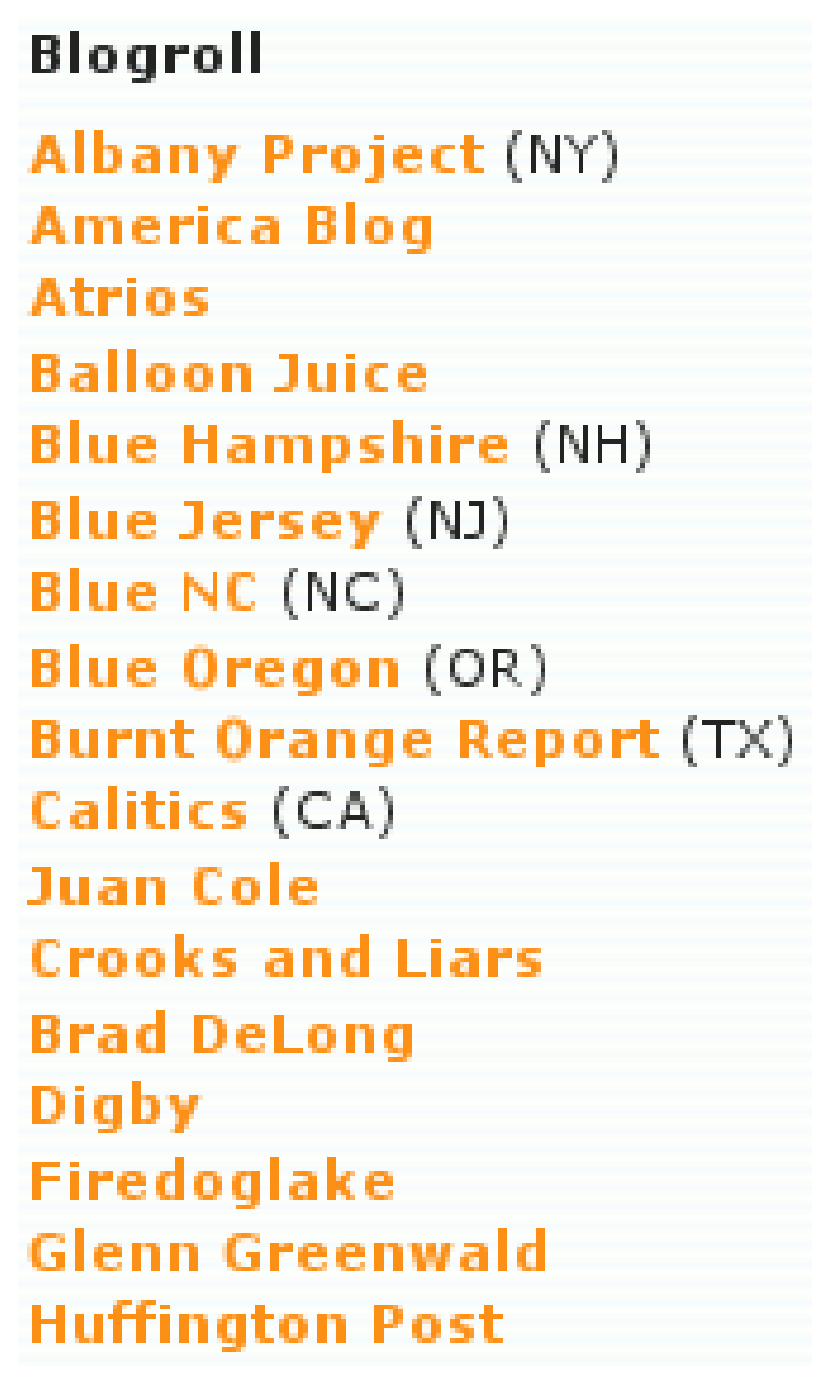
\includegraphics[width=0.9\marginparwidth]{scrsh_dailykos_blogroll}
}

As \citet[\p{806}]{dieberger97} argues the Web's growth, even at it's modest
size of 1997 compared to it's staggering size over 10 years later, have
implications on how easily it is to locate information. By creating pointer
pages, and now socially shared bookmarking services, users are imposing a
structure on the web. By navigating these kinds of interlinked hyperlink
collections it could be that users are getting access to more related and
higher quality information. Sharing a hyperlink, either on you web page or
trough a bookmarking service, requires a conscious effort. One would believe
that people only choose to do so for information they find interesting.

\subsubsection{Item Annotation}

In addition to being a modern form of pointer pages, social bookmarking
with del.icio.us introduced a new way to annotate all kinds of
items (photos, articles, wine, books, videos, music, and so on).
By applying textual key words to
bookmarks\dash{}and later other types of content\dash{}users were able to
browse such collections in new ways. These key words have been popularized as
\term{tags} and the act of applying them is called \term{tagging}%
\sidenote{
  Tagging was discovered by Joshua Schachter when he kept a plain text file
  with a list of all his web page bookmarks. He annotated these bookmarks by
  introducing single-worded labels prefixed with a number sign (\#). He could
  then easily search his bookmarks file with these labels by prefixing
  searches with the number sign. Schachter later introduced tagging to the
  masses by creating the del.icio.us social bookmarking site
  \citep[\p{92}]{weinberger07}.
}.
Joshua Schachter, the creator of del.icio.us, highlight tagging as it's most
essential feature\dash{}the feature that set it apart from the competition
\cite[\p{225}]{livingston07}. Tagging solves a recurring problem with
using traditional folder or hierarchical categorization of items like
bookmarks. In such a system an item can only go in one folder. With
tags items can live in several categories at once
\citep[\p{93}]{weinberger07}.

Tagging enables a user driven taxonomy (classification)
which is often called an \term{folksonomy}\dash{}a combination of the words
\emph{folk} and \emph{taxonomy}. A folksonomy is a strictly bottom-up
approach because of the lack of any predefined taxonomic structure. They
therefore rely on \postquote[\p{31}]{marlow06}{%
  shared and emergent social structures and behaviors, as well as related and
  linguistic structures of the user community}
Since we're mainly interested in the navigational possibilities tagging can
give us we're leaving out a deeper discussion of the benefits and drawbacks
of folksonomies. \citet{golder06} and \citet{marlow06} gives a detailed
account of the tag usage and structure in respectively del.icio.us and
\project{Flickr}%
\sidenote{%
  Flickr is a social image sharing web site available at
  \url{http://flickr.com}. We dig deeper into Flickr when
  we analyze it's social navigation capabilities in
  \sectionref{analysis.flickr}.
}.

As we've described tagging is often a collaborative process. Some web pages
for instance give suggestions for tags if the item you're annotating have
been tagged by others previously. Based on our own usage of collaborative
tagging system we seem to be more inclined to use some or all of these tags
than to come up with their own. In other words our vocabulary is influenced
by the user community. \citet[\p{186}]{sen06} confirmed our personal
observations when they found that the community influence affects the
vocabulary of tags an individual uses. \citet[\p{355}]{farooq07} conducted
similar studies on a collaborative tagging service where the user interface
did not display the tags other people had applied for a similar resource.
They did not find any significant reuse of tags from other users and explained
this discrepancy with the lack of visualization of other user's tags as
evident in other bookmarking services. This means that one can influence
the tag vocabulary of users when they are applying tags by showing other
user's vocabulary usage.

In addition to being shown other people's tags when tagging one can also
be given a list of the tags oneself have previously used.
Under such circumstances \citet[\p{185}]{sen06} found that the probability
of using a previously used tag rose as the amount of tags the user had
applied increased. \citet[\p{355}]{farooq07} validated this phenomena
by showing similar results from another collaborative tagging system.

Applying your own tags for a given resource makes sense if you're annotating a
bookmark. You have your own representation of the bookmark given by the name
you gave it and the tags you chose to apply. Since a bookmark is distinguished
by a \abbr{URL} others can have other representations of the same resource.
For other content items as photos in a photo sharing site it may make more
sense to allow every user, not only the creator, to apply globally visible
tags for this single item. There is then only one representation of this item
and it's tags.
Tags need not be collaboratively created. When one for instance are tagging
one's personal email messages it makes sense to keep such behavior private.

As we've seen folksonomies can be separated by their level of tag sharing
(private systems, fully open systems, and systems with user control over
what gets shared) and tag scope (are tags applied to an item globally
or do they belong to separate users).
\citet[\pp{34}{36}]{marlow06} gives a very detailed account of how tagging
systems can differ in design and how such variations can result in
folksonomies with different characteristics.

Annotating items seems to have benefits with regards to describing the items
and use them for categorization. But how does this relate to navigation?
By giving users a means to better describe various items it will hopefully be
easier for others to use this information in navigation\dash{}they will
hopefully easier find the items or resources they are searching.

The seemingly most used way to display tags for navigation is by generating
a so called \term{tag cloud}%
\sidenote{
  According to \citet{wikipedia08tagcloud} the first usage of tag clouds
  was on Flickr for showing tags applied to photos. The idea of such
  visualization seem to have come from \citet{flanagan03}'s display
  of search terms used when accessing his web site.
}.
\prequote[\p{1}]{fokker06}{%
  succinctly defines the technique as}{%
    The cloud is a representation of the frequency-based relation of tags}


\citet{jarrett05} gives an account into how they created a syndication
aggregator with tagging support. They designed their application with a focus
on enabling users to easily find relevant syndication items trough
social navigation. The cornerstone of their approach to social navigation was
enabling a folksonomy the users could navigate for finding syndication
items. Sadly user studies and evaluations
of the merits of this approach to social navigation is non-existent.

\citet{millen06} on also gives an account of how they used collaborative
tagging with a focus on enabling social navigation in their
\project{Dogear} social bookmarking system. Fortunately they have conducted
studies on the merits of such an approach to social navigation. When users
were navigating bookmarks they most frequently browsed bookmarks for a given
user. But browsing by a tag was not much less frequent, supporting evidence of
the usefulness of folksonomies for enabling social navigation. In addition
it was found that of all bookmarks clicked, 74\% was of other user's
bookmarks, a degree the authors interpret as evidence of a high degree of
social navigation within the social bookmarking system.

\citet[\p{1}]{fokker06} argues that collaborative tagging is ideal
when you have objects where one can not easily perform keyword search on the
information it contains. If these objects are composed of video content tags
can serve as an augmenter for performing keyword based searches as one could
do in textual content. They leveraged tagging in this manner when creating a
prototype of Wikipedia supporting video content\dash{}using tags as the
principle navigation mechanism. By doing so \citet[\p{2}]{fokker06}
saw the need for bootstrapping the availability of tags so that users would be
more inclined to create their own tags. Their solution was to algorithmically
create tags based on the contents of Wikipedia and hoped the existence of
these tags would stimulate users to start tagging themselves.

Tagging have it's shortcomings. Tags could be misspelled, tags with the same
name are not always  homonymous, and tags with the same meaning does not
always have the same name because of synonyms \citep[\p{59}]{aurnhammer06}. In
addition \citet[\p{943}]{li07} argues that browsing tags by traditional
methods with keyword search or tag clouds is inefficient when the set of tags
are quite large. They implemented a system to mediate the synonymy and
homonymy problems with tags in addition the the problems with browsing a large
collection of tags. Their solution to tag ambiguity
was to generate the semantic concept%
\sidenote{
  Generating the semantic concept of a tag means to derive it's meaning in
  a broader sense. Say for instance that a user is browsing for
  \emph{movies}. An algorithm that generates the semantic meaning of
  \emph{movies} could for instance map this to the concept of \emph{movie},
  where such tags as \emph{movies}, \emph{film}, and \emph{flick} could be
  associated with the concept of \emph{movie}.
}
of a tag and use that semantic meaning
when the user is looking for resources through tag browsing
\citep[\p{946}]{li07}. As \citet[\p{95}]{weinberger07} argues this problem
with tag ambiguity does not really matter when the collection of annotated
items becomes sufficiently large. One would only be concerned with such
matters if one need to find every possible item that is associated with a
concept.
The problem of browsing large scale tagging collections is tackled by
inferring a hierarchy%
\sidenote{
  Once can tag object by several levels of abstraction. One can for instance
  tag a movie with \emph{movie} to identify what it is. Then one could use
  the tags \emph{comedy}, \emph{romanticcomdey}, and \emph{norwegian} for
  describing the object's features. One could computationally derive an
  hierarchy from the varying levels of abstraction in such tags saying
  that \emph{comedy} is the child of \emph{movie} and \emph{romanticcomedy}
  is the child of \emph{comedy}.
}
from the flat tag space \citep[\pp{946}{948}]{li07}.

We've seen that item annotation or tagging can be used to annotate items for
describing the information they convey and
thereby afford navigation. As we'll see in
\sectionref{background.social.navigation.applied.forms.recommendations}
annotations can also be used for describing the quality, importance, or
usefulness of an item and thereby potentially creating recommendations.

\subsubsection{Interaction History Trails}
\label{section:background.social.navigation.applied.forms.interaction.history}
% in the wild: trail-fire, new hoodwink.d like Greasemonkey service
% history-rich objects: hill92, hill94

In a classic article \citet{wexelblat99} contrasts the digital world of
computers with our physical world with respect to the formers lack of history.
In our traditional world we exploit such historical information traces
\postquote[\p{270}]{wexelblat99}{%
  to guide our actions, to make choices, and to find things of
  importance or interest}
It's argued that this apparent lack of history in computerized systems must
be sorted out such that future users can take advantage
of past users' historical traces left when they were working
on solving problems similar to the current user's.
A possible remedy for this problem on the Web is put forth in the authors'
\project{Footprints} system\dash{}an navigational aid as an extension to
normal web browsers, visualizing interaction history of past users enabling
current users to navigate this history.

This interaction history consists of several navigation trails which are
\postquote[\p{273}]{wexelblat99}{%
  coherent sequences of nodes followed by an individual}
The idea of such trails of navigation far preceded \citeauthor{wexelblat99}
as they were envisioned by \citet{bush45} when he proposed the infamous
theoretical computer-like system named the \project{Memex}%
\sidenote[-15\onelineskip]{
  The Memex was not envisioned as a computer system but as an
  mechanical system consisting of a set of controls hooked up
  to a microfilm reader and camera. It was
  theorized by \citeauthor{bush45} to be a system for handling
  a persons entire collection of documents, books, and communication.
  It was
  important that a user would be able to access this information with great
  speed and flexibility. An integral part of enabling such efficient access
  was a user' and content providers' ability to introduce trails between
  information items. \citeauthor{bush45}'s writing about trails
  inspired hypertext \citep[\p{86}]{nelson65} which in turn was the grand idea
  behind the World Wide Web \citep[\p{49}]{myers98}.
}.
\citeauthor{bush45} describes a scenario where users are building trails
explicitly, inserts comments if needed, and gives it a name.
\citeauthor{wexelblat99} on the other hand
implemented a system where trails are automatically collected using a set of
heuristics to identify browsing behavior representing a coherent navigation
trail.
\citeauthor{bush45} wrote his essay before the invention of computer networks
and he thinks of each Memex as a separate island. Sharing of trails is
possible trough an exportation and following importation process, making it an
explicit action for it's users.
The Footprints system makes the social process of sharing trails implicit and
transparent to it's users\dash{}multiplayer is forced.

Controlled user studies by \citeauthor{wexelblat99} did partially falsify
their pre-test hypothesis of Footprint's ability to let users find more
relevant results during a specific browsing task and that this browsing
would be more efficient. The group using the history-enriched system reported
significant lower values of mean page count in their browsing task. No
significantly difference in results returned was found between users of a
plain web browser and users with a browser enhanced with Footprints. They also
found that people experienced in the problem domain of the browsing task were
to a larger degree able to take advantage of interaction history than novices.
\citeauthor{wexelblat99} attributed this to experienced people's ability to
have a clearer mental model of the information one was browsing.

% Juggler discourse here, maybe

\subsubsection{Populated Space}

A \term{populated space} is
\postquote[\p{41}]{dieberger00b}{%
  an information space in which other people can be encountered}
By providing online awareness users can see where other users are moving and
spending time. In contrast to interaction history where such behavior is
stored for later retrieval a populated space only shows what others are doing
in real-time.

\project{Kalas} \citep{svensson05}, a system for interacting with food
recipes, uses the idea of populated space to enable user awareness. Kalas is
also a recommendation system and is in our opinion one of the best studied
social navigation systems. We'll therefore come back to
\citeauthor{svensson05}'s evaluations of different social
navigation techniques.

\subsubsection{Collaborative Filtering}
\label{section:background.social.navigation.applied.forms.collaborative.filtering}
% introduce earlier cited goldberg92 article and more recent work.
% collaborative filtering is often used for recommendation systems
% look at the benefits of implicit feedback in contrast to explicit feedback
% with regard to recommendation systems as highlighted by claypool01.

\todo{Discuss the most important articles and implementations.}

\subsubsection{Recommendations}
\label{section:background.social.navigation.applied.forms.recommendations}

So called \term{recommender systems} are often based on collaborative
filtering principles. % continue discussion and citing.

One of the two forms of social navigation found in
\project{Knowledge Sea}\dash{}a digital educational
library\dash{}is recommendations by item
annotation \citep[\p{13}]{brusilovsky05}. Users can leave their emphatic marks
on content and thereby specify it's usefulness. Questionnaires showed that a
fair majority of users was agreeable to the use of such recommendations
\citeyearpar[\p{15}]{brusilovsky05} and log analysis strengthened
the impression
\begin{fullquote}[\p{38}]{brusilovsky05}{had by showing that}
  Social navigation support and specifically
  annotation-based social navigation increases the chance of
  accessing a resource dramatically.
\end{fullquote}

Advanced algorithms known in the field of collaborative filtering
and recommendation systems have been used together with folksonomies
consisting of collaborative tags
\citep[\pp{112}{113}]{wu06}. Preliminary studies have shown positive
results when harnessing such social knowledge with filtering algorithms
as opposed to traditional folksonomy representation
\citep[\p{114}]{wu06}. Such a folksonomy could hoverer interfere with an
existing recommendation system. \citet[\p{190}]{sen06} found that the
introduction of tagging and tag display in their established
movie recommendation system interfered with some of the users primary
objective: finding interesting movies. Note that this dislike of a
folksonomy was more likely to be present for users familiar with the old
movie recommendation system sans any folksonomy. New users having not
witnessed the recommendation system without any folksonomy seemed more
acceptant towards tagging.

\subsubsection{Social Texture}
% activity, usage, edit/read wear
% footprints users edit/read wear for instance.

\begin{figure}
  \captionstyle{\raggedright}
  \begin{whole}
    \begin{minipage}[t]{0.475\wholewidth}
      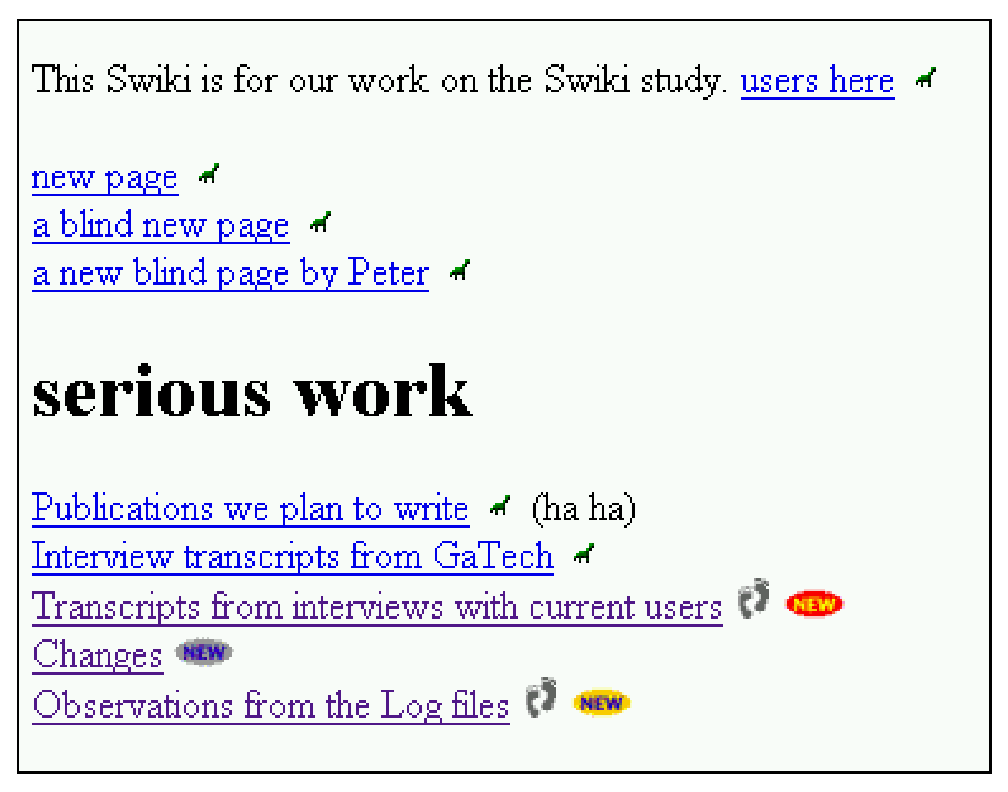
\includegraphics[width=\textwidth]{scrsh_coweb_contextual}
      \caption[CoWeb Contextual Cues]{%
        CoWeb Contextual Cues,
        retrieved January 25, 2008, from
        \url{http://homepage.mac.com/juggle5/WORK/publications/SwikiWriteup.html}.
      }
      \label{figure:scrsh.coweb.contextual}
    \end{minipage}
    \hfill
    \begin{minipage}[t]{0.475\wholewidth}
      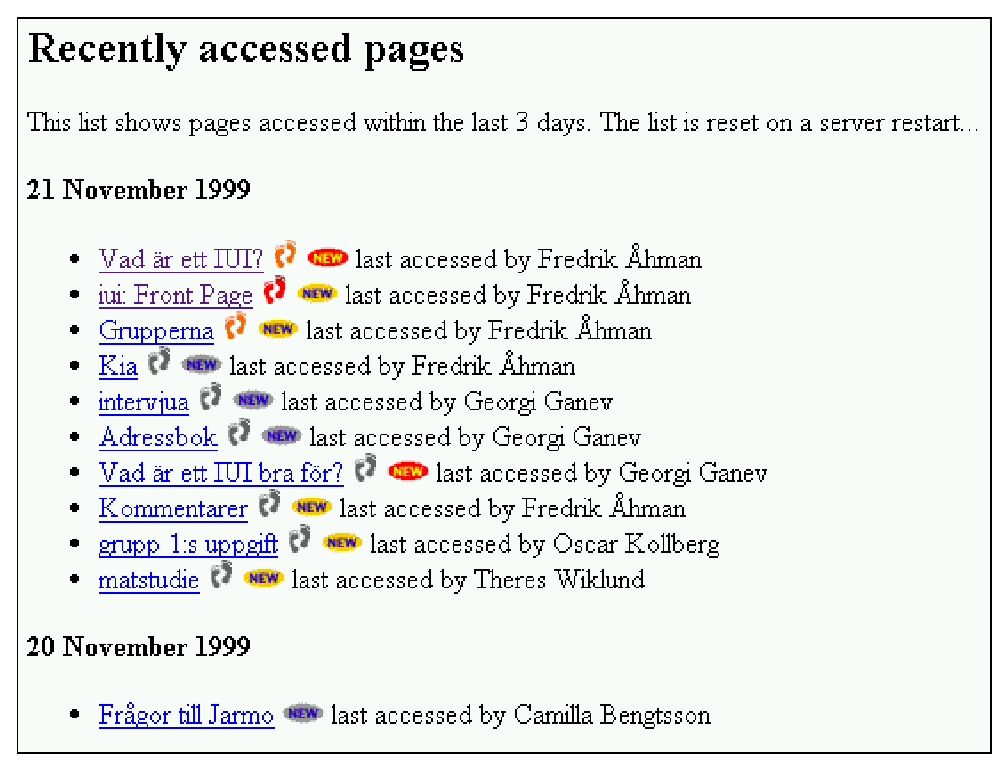
\includegraphics[width=\textwidth]{scrsh_coweb_global}
      \caption[CoWeb Global Cues]{%
        CoWeb Global Cues,
        retrieved January 25, 2008, from
        \url{http://homepage.mac.com/juggle5/WORK/publications/SwikiWriteup.html}.
      }
      \label{figure:scrsh.coweb.global}
    \end{minipage}
  \end{whole}
  \normalcaption
\end{figure}

We use \term{social texture} to describe socially constructed annotations or
visualizations which may be used for navigation or in some form guide
users in navigational choices.

Social texture ties in with the forms of social navigation we've
recently discussed. Tagging for instance is a social texture.
The interaction history systems we've discussed uses forms of visualizations
in close proximity to hyperlinks to convey their degree of usage. This is also
a form of social texture.

The first forms of social texture used in computer systems to our knowledge is
\citet{hill92}'s usage of \term{computational wear} which is an analogy for
the wear physical objects experience when used. They modify a text editor to
show both wear related to document edits and readings of documents. This wear
is graphically visualized trough the editor's scroll bar.
The concept of edit and read wear has since been used on the Web in for
instance the Footprints system \citep{wexelblat99}.

\citet{dieberger00a} modified \project{CoWeb}\dash{}a collaborative Web space
modelled after Ward Cunningham's famous Wikis\dash{}to include interaction
history visualization hoping to make it a more social space, enabling social
navigation. They visualized other users' access of different pages both by
including a global list of such behavior and contextual cues about access
next to internal hyperlinks.
It was inferred by \citeauthor{dieberger00a} that markers of interaction
history increased the overall activity on the web page during a user study.
They also learned that it's important to both provide both global and
contextual interaction history cues.

\citet{xu06} modified a Wiki in even more elaborate ways
with the aim of integrating several social navigational mechanisms.
They used read-wear information for creating social
texture in the Wiki both in-line pages, on a page level, and on a global
level. \citeauthor{xu06} took the approach of displaying read-wear in real
time, thus making the system a populated space. To make such an approach
useful the Wiki needs a certain amount of users present at all times. If
it's not frequently trafficked it would probably be better to represent
historical read-wear as done in CoWeb \citep[\p{220}]{dieberger00a}. Both
contextual and global use of such social texture can be seen in
\figureref{scrsh.coweb.contextual} and \figureref{scrsh.coweb.global}.

\project{virtPresenter} is a hypermedia based lecture viewer where read-wear
have been used to visualize a groups' interaction with continuous content
\citep{mertens06}. By following the traces other users have left current users
can interpret what's the most sought after parts of a lecture. The
visualization is implemented in ways similar to \citet{hill92} by showing
graphs of usage in line with a timeline selector and can be seen in
\figureref{scrsh.virtpresenter.timeline}.

We discussed KnowledgeSea regarding it's use of recommendations in
\sectionref{background.social.navigation.applied.forms.recommendations}.
The system also incorporates what the authors calls
\term{traffic-based social navigation}
\citep[\p{12}]{brusilovsky05}\dash{}in other words history based
visualizations in the form of read-wear. The access of different articles in
the digital library are recorded and the degree of usage is then visualized in
the form of different color tones where darker indicates a more popular
resource. Such visualization is used consistently throughout the web site. A
questionnaire revealed that in excess of 70\%
\citeyearpar[p.15]{brusilovsky05} of the users
found such history based visualizations useful and appropriate.

\begin{figure}
  \centering
  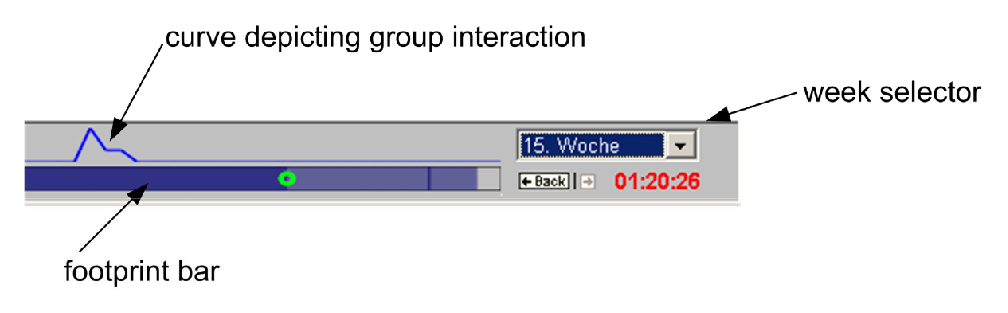
\includegraphics[width=0.9\textwidth]{scrsh_virtpresenter_timeline}
  \caption[virtPresenter Timeline]{
    virtPresenter Timeline \citep[\p{43}]{mertens06}.
  }
  \label{figure:scrsh.virtpresenter.timeline}
\end{figure}


\subsubsection{Search}
% social search articles and semantic web/search article
% not that relevant as we're focusing on navigation trough browsing
% brusilovsky05 have some discussion of using social navigation in search
% results

\subsection{Usefulness}
% dieberger00b:
%   filtering: HEE - find most relevant info
%              RecSys - pick items from a large space
%   quality:   HEE - find quality info (interesting, valid)
%   social affordance: HEE - users aware of each other
%                          - social experience
%                      - space is alive
%                        - not only affect navigation
%                          - stay longer in the space
%                          - relaxed
%                          - try new features

\citet{svensson05} performed a throughout evaluation of the Kalas system and
two issues in perspective of social navigation:

\begin{enumerate}
  \item Will social navigation enable users to navigate more efficiently?
  \item Do social navigation increase the perceived subjective quality of
    a navigation process?
\end{enumerate}

Server logs were statistically mined and more in depth qualitative interviews
were conducted. The results showed that people tended to move to the most
populated part of system and used recommendations for helping select which
items to navigate. \citeauthor{svensson05} also found that the subjects
overall had a positive impression of the social features of the system. They
seemed more interested in expressing themselves trough such features than
using information from others to help their navigation process.

Favorable results for the effectiveness of social navigation was observed
during a simulation experiment conducted by \citeauthor{riedl03}. In most
circumstances social navigation had favorable results in efficiency contrasted
with asocial navigation. It's important to note that social navigation
decreased the effectiveness of navigation in some instances of their
simulations \citeyearpar[\p{365}]{riedl03}.
Interestingly, it was discovered that social navigation was more
beneficial in environments with high uncertainty%
\sidenote[-5\onelineskip]{
  \prequote[\p{363}]{riedl03}{%
    says that the two sources of such uncertainty is}{%
      arising from the correctness of the information gained in any state,
      and the potential difficulty of reaching that state to obtain
      the information}
}
than environments with higher certainty\dash{}provided that the
simulated agents could reach the social media
\citeyearpar[\p{368}]{riedl03}. 

\section{Building on Top of the Web}
\label{section:building.on.top.of.the.web}
% Greasemonkey, hoodwink.d, new hoodwink.d service
% browser extensions related, Greasemonkey itself a extension, but
% thinking about specialized plugins for enabling interaction on top of other
% web pages.
% mashups kind of related, maybe put inside web2.0 part or separate part
% open apis is the fuel for mashups. possible without by screen scraping, but
% not as convenient and safe (upgrades on the pages we're scraping)
% facebook, open social. applications on top of social network sites.
% installed base of users and relationships already in place.

Going in and making changes to an existing web site can be both an
daunting and time consuming task. First one have to establish a trustworthy
relationship with the creators of such a site so that they are certain
you're not introducing bugs in their production software. Secondly, grasping
the code base, third party libraries, and development tools of such a software
project demands a lot of upfront effort before any real development work can
begin. This goes against the prototypical process we intended to use while
experimenting with \urort{}.

Even though we've had an ongoing dialog with the developers of \urort{} we
decided to create our prototype as a layer on top of their site.
By using an
extension
for the leading open source%
\sidenote{
  The \project{Firefox} web browser. Available at \url{http://firefox.com}.
}
web browser we were able to create a script which
made changes and additions to the way \urort{}
were presented to users who were participating in our study.
Such an approach would hopefully result in a transparent experience for our
end users as long as they have taken the necessary steps to set up the browser
extension and our script.

The idea of creating additional features for a web site in these manners
came from the author's involvement in an underground community based around
the Ruby%
\sidenote{
  Can be retrieved from \url{http://ruby-lang.org}.
}
programming language. \project{Hoodwink.d}%
\sidenote{
  Hoodwink.d's starting point for new users can be seen
  at \url{http://hoodwinkd.hobix.com}.
},
as it's called, is a service that lets members post comments on all kinds of
web sites. These comments are then only visible to the members of the
community.
Hoodwink.d is underground in the sense that it's quite hard to get in to
the community. It's members rarely talk about Hoodwink.d publicly, baring
similarities to the underground fight club in a novel by \citet{palahniuk96}
aptly named \work{Fight Club}%
\oddsidenote[-4\onelineskip]{
  The first two rules of this underground club in the novel of
  \citet[\pp{48}{50}]{palahniuk96}
  clearly describes the attitude members have to outsiders:
  \begin{inparaenum}[(i)]
    \item You don't talk about fight club.
    \item You don't talk about fight club.
  \end{inparaenum}
}.
The home page of Hoodwink.d mimics the community's dedication to secrecy
by obfuscating it's information as can be seen in
\figureref{scrsh.hoodwinkd.obfuscation}.
When the information on the page is viewed without obfuscation%
\oddsidenote{
  The obfuscation can be removed either by turning off \abbr{CSS} support
  in your browser or viewing the page's source.
}
one have to be pretty technical savvy to decipher what the information 
actually means. Simply put users have to change their hosts file
so that it points to two imaginary domain names. Doing so they can point their
browser to these domains and download a script (such scripts are discussed in
\sectionref{selection.stack.client.platform})
that enables the functionality
of Hoodwink.d.%
\oddsidenote{
  Oh no, we just broke the first and second rule of \work{Fight Club}!
}
This approach creates a barrier to entry which only allows the most
technically inclined to enter the community\dash{}allowing for a
high level of technicality in the community's internal discussions
and thereby filtering out so called \term{newbies}
(newcomers and beginners).

\begin{figure}
  \centering
  
\includegraphics[width=0.9\textwidth]{scrsh_hoodwinkd_obfuscation}
  \caption[Hoodwink.d Obfuscation]{
    Obfuscation of Hoodwink.d's home page,
    retrieved March 6, 2008, from
    \url{http://hoodwinkd.hobix.com}.
  }
  \label{figure:scrsh.hoodwinkd.obfuscation}
\end{figure}

\begin{figure}
  \begin{whole}
    \centering
    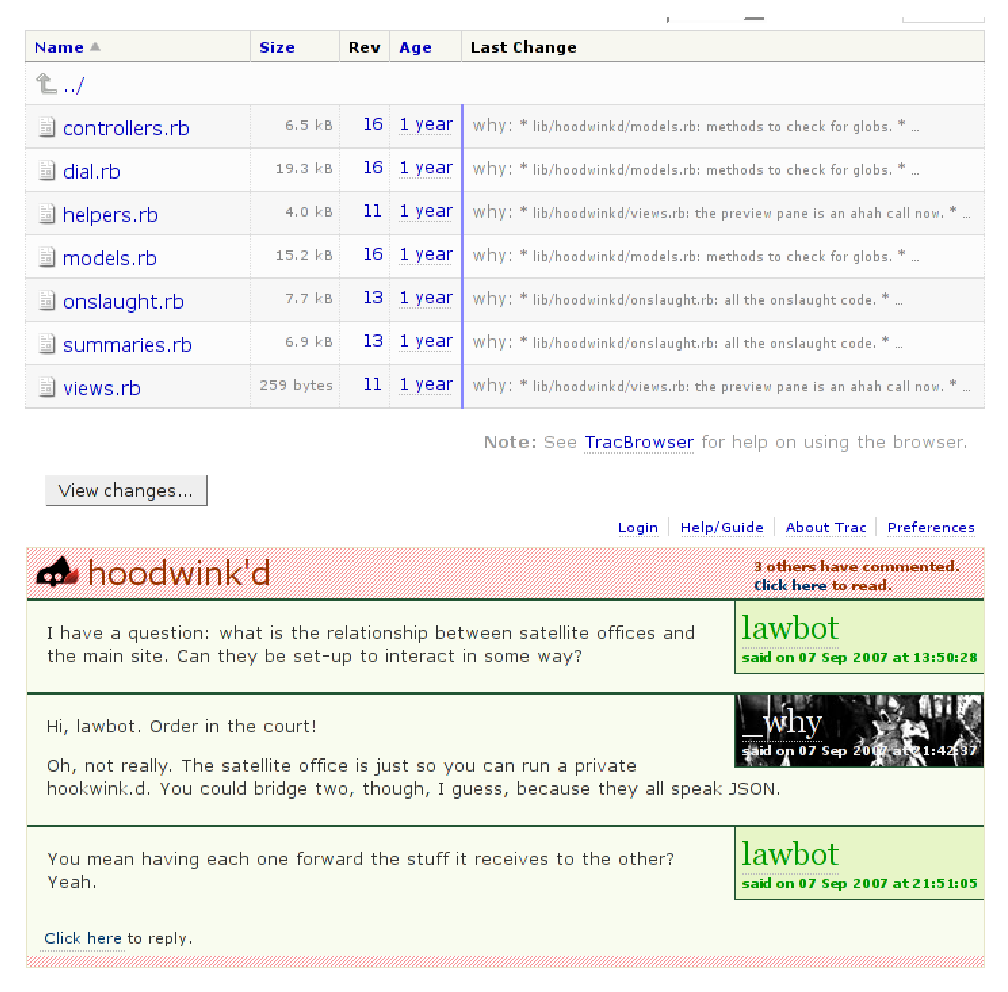
\includegraphics[width=0.9\wholewidth]{scrsh_hoodwinkd_comment_source}
    \caption[Hoodwink.d Comments]{
      Comments on the repository browser of Hoodwink.d's source code,
      retrieved March 7, 2008, from
      \url{http://code.whytheluckystiff.net/hoodwinkd}.
    }
    \label{figure:scrsh.hoodwinkd.comment.source}
  \end{whole}
\end{figure}

Now we finally get to the really interesting part of Hoodwink.d: the features
it enables on top of the Web. One can create a comment visible only to the
community's members on any web page that is supported. This support is not
dependant on the creator of the web site, but the users of Hoodwink.d needs to
record some information of the web site (where the comments should be placed)
to make it supported. \figureref{scrsh.hoodwinkd.comment.source} shows an
example of how these comments are displayed on the repository browser for
the Hoodwink.d source code itself. This page does not natively support
comments. Using Hoodink.d for such means is a very cheap (time wise) option
compared to implementing such features in the repository browser.
They are perceived as being part of the web page itself, even though they
are inserted right after the page is fully loaded.

To tie together these comments a central portal lists
the most recently placed comments (as can be seen in
\figureref{scrsh.hoodwinkd.onslaught.recent}), the most actively commented web
sites, the most recently new supported sites, and the most active users.

\sidefigure{Hoodwink.d Recent Comments}{%
  Recent comments on Hoodwink.d,
  retrieved March 7, 2008, from
  \url{http://hoodwink.d/onslaught}.
  \label{figure:scrsh.hoodwinkd.onslaught.recent}
}{%
  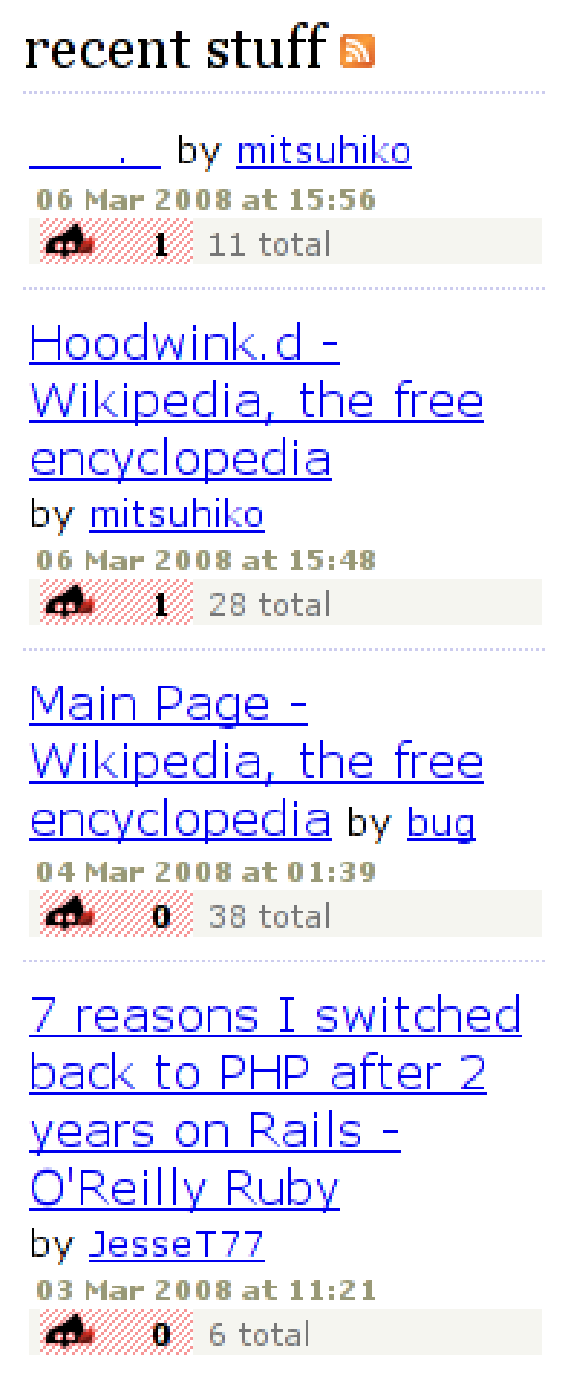
\includegraphics[width=0.9\marginparwidth]{scrsh_hoodwinkd_onslaught_recent}
}

    \chapter{Methodology}
\label{chapter:methodology}

This chaper will include information in how data was collected. So far this
includes content inventory/analysis.

\section{Content Analysis}

The term \emph{content analysis} is most often used to signify a research
technique used in the social sciences.
\citet[p.~18]{krippendorff03} defines it as:
``a research technique for making replicable and valid
inferences from texts (or other meaningful matter) to the contexts of their
use''.

This is however not the use of the term we're concerned with here. We consult
content analysis as the more pragramtic practice conducted within the field of
\emph{information architecture}%
\sidenote{
  \citet[p.~4]{morville06} defines information architecture as:
  \begin{inparaenum}[(a)]
    \item the structural design of shared information environments,
    \item the combination of organization, labeling, search, and navigation
      systems within web sites and intranets,
    \item the art and science of shaping information products and experiences
      to support usability and findability, and
    \item an emerging discipline and community of practice focused on bringing
      principles of design and architecture to the digital landscape.
  \end{inparaenum}
}.
Content analysis is deployed as a technique by information architects for
helping them generate a sound and well structured web site architecture.
It consists of two phases:
\begin{inparaenum}[(i)]
  \item a collection of a representative sample of data and
  \item an analyses of this collected data
\end{inparaenum}
\citep[pp.~241--243]{morville06}.
A graphical content mapping can be included as an optional
intermediate phase between data inventory and analysis if one finds such
representations helpful for understanding a web site's structure.
In it's essence a content analysis should identify the various
relationships (or lack of correlation) between a web site's content items.

Instead of using content analysis as a means for improving on an existing
site's content architecture we'll be tailoring this technique to best help us
discover and understand social navigation patterns in infamous web sites which
are known to make good use of such navigational designs.

    \chapter{Analysis of Social Navigation in Modern Web Sites}
\label{chapter:analysis}

This chapter will include a survey and analysis of the data we've collected
which can be found in it's whole in
\appendixref{content.inventory}.

\section{Flickr}

\sidefigure{Flickr Photo Meta-data}{%
  Photo Meta-data,
  retrieved October 28, 2007, from
  \url{http://flickr.com/photos/benbengraves/187609810/}.
  \label{figure:scrsh.flickr.photo.detail.metadata}
}{%
  \includegraphics[width=0.9\marginparwidth]{scrsh_flickr_photo_metadata}
}

Flickr is a photo sharing site which are known to be on the cutting edge when
it comes to enabling new and innovating features in it's domain. Flickr has a
quite peculiar history as it started out as a massively multi player online
game. An environment for photo sharing within the game was added in 2004 which
quickly became more popular than the game itself. The focus of the company was
shifted and their new photo sharing community was bought by Yahoo! Inc. in
March 2005 \citep[p.~257]{livingston07}.

This subsequent
analysis of Flickr will be carried out as a registered user. One has to be
registered for interacting with the site in such a way that one leaves
persistent traces. The site has a open nature enabling anonymous access
to the majority of content.

\subsection{Thumbnails}

Already on the welcome page (\figureref{scrsh.flickr.welcome})
we're finding navigation links that are social of
nature. Four thumbnails functions as sample of the most recently uploaded
photos by other members of the community. One can either navigate straight to
a detailed page for each particular photo by clicking on the respective
thumbnail (Id 6, p.~\pageref{table:flickr.content.inventory.6})
or the profile of the uploader by clicking on their user
name (Id 7, p.~\pageref{table:flickr.content.inventory.7}). Such thumbnails
with minimal meta data (the uploader) are prevalent all over Flickr. Of the
120 pages we collected in our content inventory 26 of them contained
thumbnails. Most of these thumbnails
are giving users incentives to navigate using social means%
\sidenote[-4\onelineskip]{
  Apart from the few pages that only show a
  stream of your own thumbnails when you're browsing your
  own photos by various methods.
}.
Which photos these thumbnails portray is dynamic. That is to say that other
users' actions\dash{}uploading a photo, tagging a photo, taking a photo with a
specific camera, collecting photos into sets, and adding photos to a certain
group\dash{}all determine the navigational choices you as a user is
presented with.

\subsection{Meta-data}

We arrive on a photo detail page as in
\figureref{scrsh.flickr.photo.detail}
if we utilize one of these thumbnails for navigation. In addition to comments
on the photo we find meta-data as in 
\figureref{scrsh.flickr.photo.detail.metadata}
Meta-data include the date the photo was taken, the manufacturer and the model
of the camera that was used which are all so called Exif%
\sidenote{Exchangeable Image File: a specification for image file format used
in digital cameras.}
data. Flickr utilize this data by enabling navigation based both on the
dates a picture was taken and by camera make and model. Say you're trying to
find a picture from your home town on a particularly beautiful summer day. By
using date of picture taking based navigation coupled with tags or
geographical data (which both will be discussed shortly) you're probably
increasing you chances of finding what you want. Camera make information could
be useful when looking at the quality of pictures taken with certain cameras
before purchasing one yourself.

\begin{figure}
  \captionstyle{\raggedright}
  \begin{whole}
    \begin{minipage}[t]{0.475\wholewidth}
      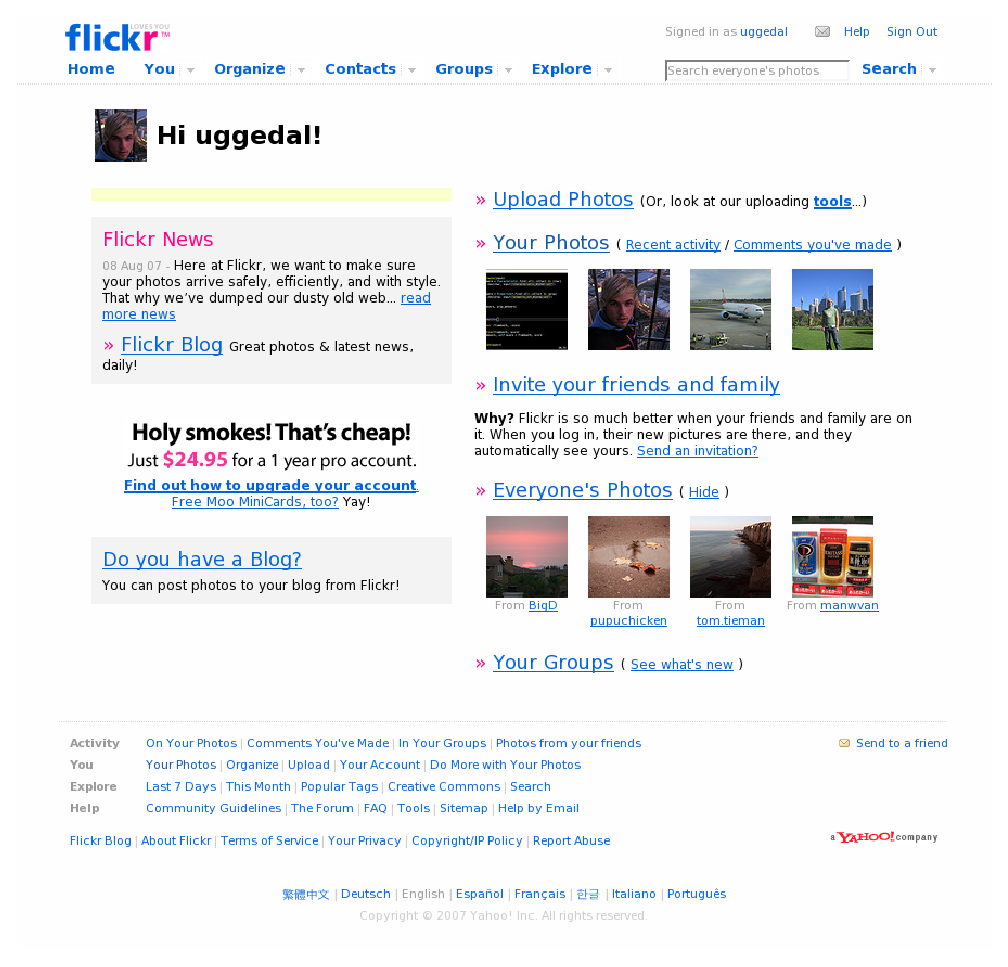
\includegraphics[width=\textwidth]{scrsh_flickr_welcome}
      \caption[Flickr Welcome Page]{%
         The Welcome Page,
         retrieved October 16, 2007, from \url{http://flickr.com}.}
      \label{figure:scrsh.flickr.welcome}
    \end{minipage}
    \hfill
    \begin{minipage}[t]{0.475\wholewidth}
      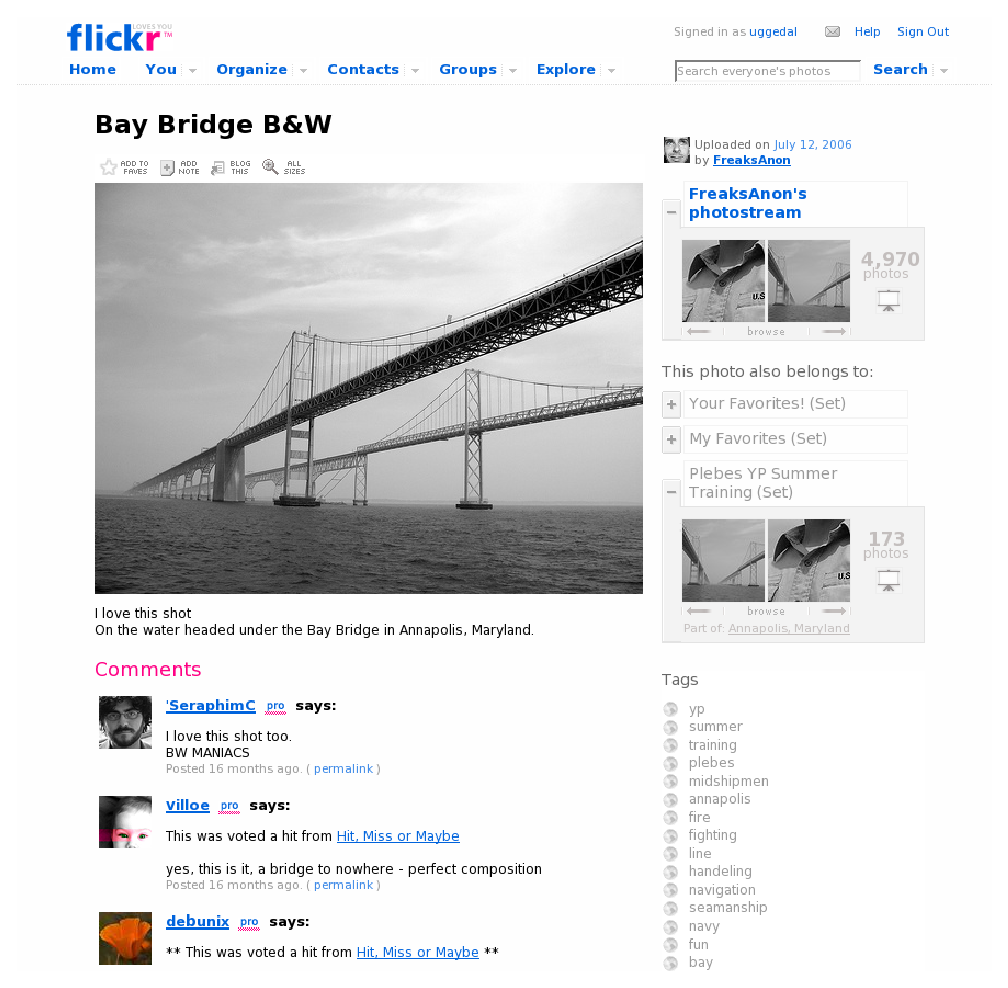
\includegraphics[width=\textwidth]{scrsh_flickr_photo_detail}
      \caption[Flickr Photo Detail Page]{%
         A Photo Detail Page,
         retrieved October 26, 2007, from
         \url{http://flickr.com/photos/benbengraves/187609810}.}
      \label{figure:scrsh.flickr.photo.detail}
    \end{minipage}
  \end{whole}
  \normalcaption
\end{figure}

\subsection{Folksonomy}
Of most importance
for Flickr, and indeed what makes Flickr a folksonomy, is it's tagging
abilities. Caterina Fake, co-founder of Flickr, explains it's importance as
\postquote[p.~261]{livingston07}{%
  Tagging really revolutionized the way the product behaved}
All registered user can label anyone's photos by applying such short
descriptive tags. This collaborative process lay the ground work for other
user's ability to easily browse photos by topic.
\figureref{scrsh.flickr.tagcloud}
exemplifies how the user generated data trough tagging can be used as a
navigational aid. A so called \term{tag cloud} is used to visualize the
popularity (and thereby importance) of the individual tags. The larger the
tag title, the more frequent the tag has been applied to photographs.

Tag clustering was released in the fall of 2005 \citep{butterfield05} as a way
to easier see the relationships between separate tags. For any given tag a
cluster of three related tags is generated and displayed to users when they
are browsing as seen in
\figureref{scrsh.flickr.photo.detail}.
Flickr algorithmically generates these listings based on what tags users tend
to use together for labeling a photo.

Tagging is a very flexible approach only hindered by users' imagination. In the
early days of Flickr there was no support for geographical data. Users soon
found a remedy for this by tagging photos with longitude and latitude. By
using the same technology we're using in our prototype application
(Greasemonkey) they were able to integrate Google Maps%
\sidenote{
  Available at \url{http://maps.google.com}
} in Flickr, enabling user's to place their photos on a map and automatically
generate geographical coordinate tags%
\sidenote{
  More info about the early days of \term{geotagging} can be found on the
  remains of the Flickr Geotagging group, available at
  \url{flickr.com/groups/geotagging/}.
}.

\subsection{Geographical data}

In late August 2006 Flickr introduced geotagging abilities
\citep{butterfield06} by integrating mapping aspects from Yahoo! Maps%
\sidenote{
  Available at \url{http://maps.yahoo.com}.
}
Users could now place their photos on a
map to signify where they were captured.
% Finish description.
% Take screen shot.
% Write about the new places feature.
% Write and cite when proper geo data was incorporated.

\subsection{Interestingness}
% Cite collaborative filtering. Introduced in same blog post as clustering.

\begin{figure}
  \begin{whole}
    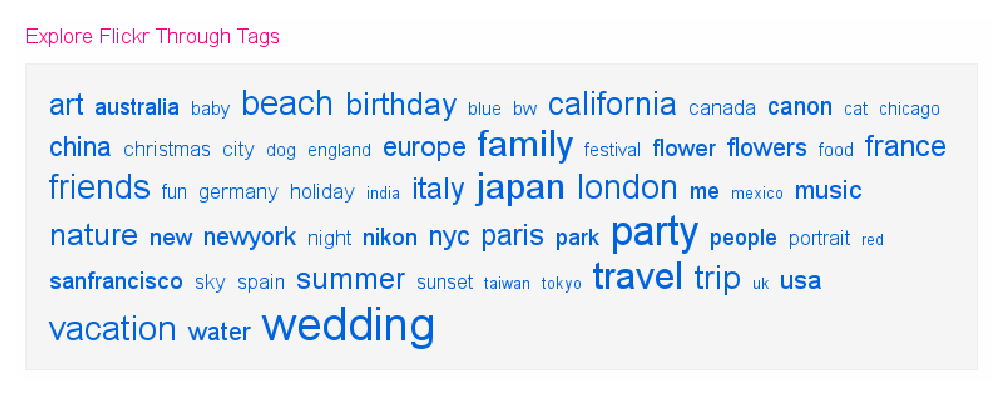
\includegraphics[width=\wholewidth]{scrsh_flickr_tagcloud}
    \caption[Flickr Tag Cloud]{%
       Tag Cloud,
       retrieved November 1, 2007, from \url{http://flickr.com/explore}.}
    \label{figure:scrsh.flickr.tagcloud}
  \end{whole}
\end{figure}

\begin{figure}
  \begin{whole}
    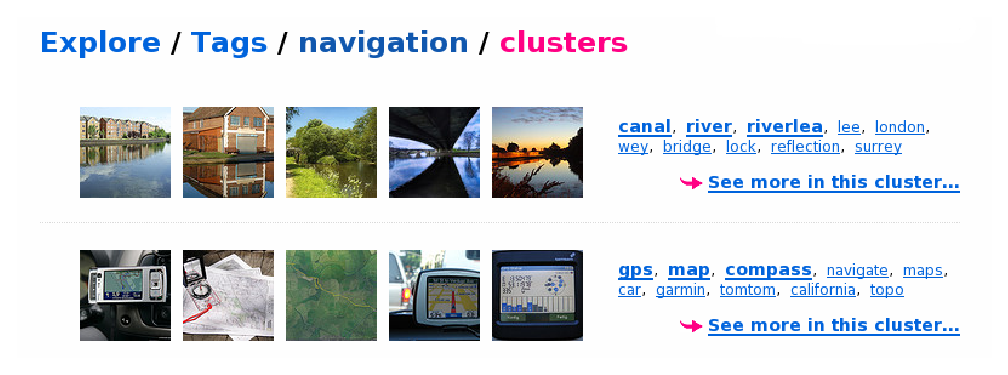
\includegraphics[width=\wholewidth]{scrsh_flickr_tagcluster}
    \caption[Flickr Tag Cluster]{%
       Tag Cluster,
       retrieved November 19, 2007, from
       \url{http://flickr.com/photos/tags/navigation/clusters/}.}
    \label{figure:scrsh.flickr.tagcluster}
  \end{whole}
\end{figure}

\section{Facebook}
\label{section:analysis.facebook}

\subsection{Profiles}

As we've seen pictures and their thumbnails and titles are central in Flickr.
In the same way user names and thumbnails of profile images are scattered all
trough Facebook. This is no mystery as the dominant entity of Facebook is
persons and their profile much as pictures' essentialness for Flickr.

\subsection{News Feed}

The landing page when you log in to Facebook after having configured your
account is a news feed. The news feed shows the recent activities your friends
have conducted.

% Include discussion of friendfeed and social thing

\begin{figure}
  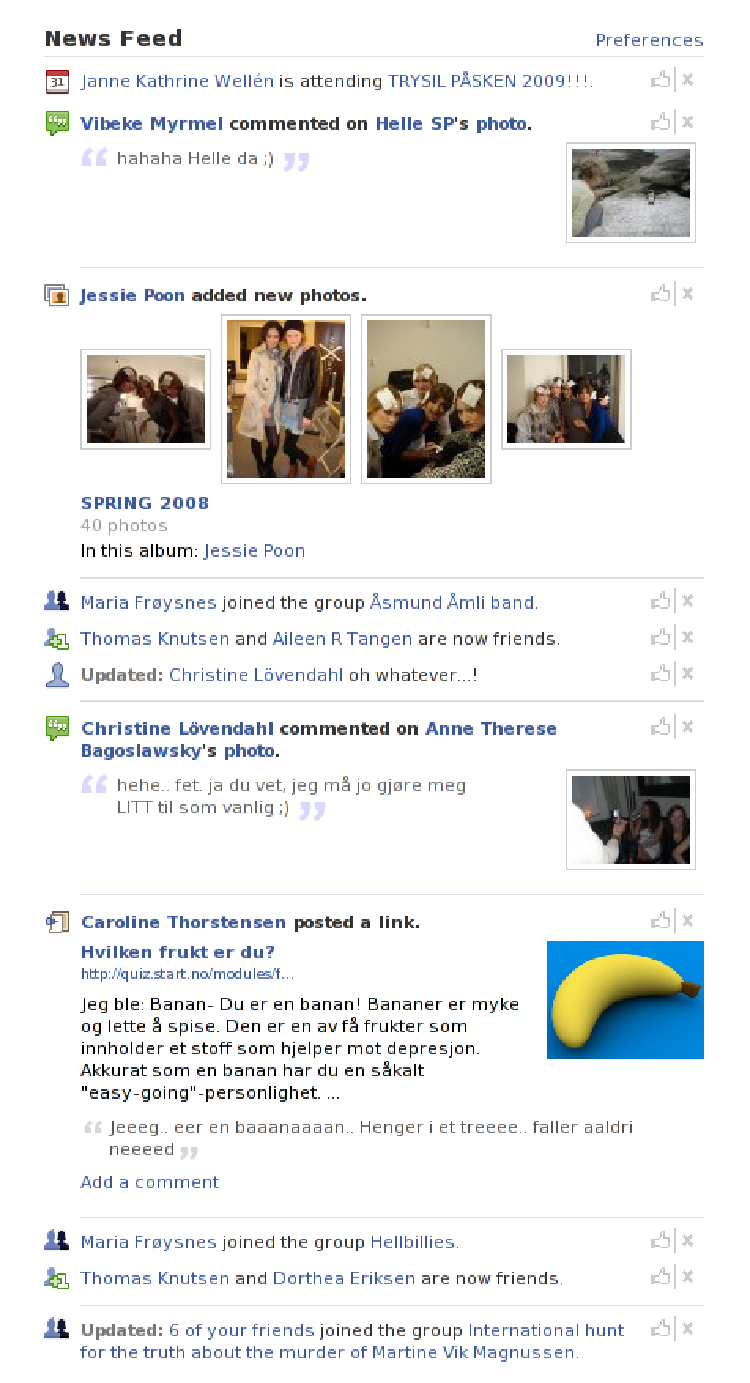
\includegraphics[height=0.9\textheight]{scrsh_facebook_news_feed}
  \caption[Facebook News Feed]{%
     News Feed on Facebook,
     retrieved March 26, 2008, from \url{http://www.facebook.com/home.php}.}
  \label{figure:scrsh.facebook.news.feed}
\end{figure}




    \chapter{Implementation}
\label{chapter:implementation}

% This chapter should include design choices for my implementation. For
% example choices taken for generating relevant data for test users
% and a computational sound method for doing so. As JavaScript in browsers are
% quite inefficient it will probably be necessary to persist data at a server
% in some sort of cache. The clients could then get this data by invoking a
% single request. The result could for instance be JSON serialized. Scraping
% of such data is probably done more efficient and safer at the server side
% since multiple XMLHttpRequests in the clients for scraping and parsing could
% prove to be quite computational expensive.

As we've seen in 
\sectionref{building.on.top.of.the.web}
it's possible to build applications on top of existing web sites by creating
transparent prototype implementations. This chapter starts with an account of
what kind of navigation system we wanted to build, goes on to describe why we
decided on such navigational designs, and concludes with an explanation of how
the implementation was built\dash{}the ingredients of our implementation.

\section{Design}

\section{Architecture}

\subsection{Client Side}

\subsubsection{Programming Language}

\subsubsection{Framework}

\subsection{Server Side}

\subsubsection{Programming Language}

\subsubsection{Framework}

\subsection{Development Tools}

\subsubsection{Version Control}

\subsubsection{Editor}

A developer's main tool for authoring software is his editor. Sometimes the
implementation language warrants a specialized editor with aids for
handeling cumbersome tasks specific to that language. Such editors is often
called \emph{Integrated Development Environments}%
\sidenote{
  A good example of an IDE is
  \emph{Eclipse} (available at \url{http://eclipse.org}).
  It was first used for Java development but since extended with
  plugins for handeling other programming languages and families.
}
(IDEs) and are used most often for languages like Java and C\#.
\citet{murphy06} found that developers mostly use IDEs for navigating large
collections of source code, refactoring code, debugging code, and interacting
with revision control systems in addition to normal editor usage.
Development environments found in Lisp%
\sidenote{
  \citet[p.~69]{sandewall78} higlights the benefits of having truly
  interactive development environments:
  ``The `residential' design of programing systems, whereby all facilities
  for the user are integrated into one system with which the user communicates
  during the entire interactive session, offers great possibilities for user
  convenience.''
}
and Smalltalk%
\sidenote{
  Similar to Lisp's programming environment
  ``Smalltalk is designed so that every component in the system that is
  accessible to the user can be presented in a meaningful way for observation
  and manipulation'' \citep[p.~viii]{goldberg83}.

}
are surpassing IDEs in integration and interactivness.

The programming languages we've deciced to work with, JavaScript and Ruby, are
very expressive and dynamic in their nature in addition to beeing interpreted
instead of compiled. Our experience is that IDE usage for such languages
stands more in the way than aid you as a programmer during your problem
solving process.


The interactive experience provided by Lisp and Smalltalk implementations are
sadly missing from JavaScript and Ruby implementations.

We're not setteling on any editor though. Developer should use the tools
that enabeles them to most efficiently and safely interact with their code
(citation needed). The editor one chooses to use should also depend on how
much time one has available to learn to use it efficently. Truly powerfull
editors are charactericed with a big up-front investment in learning.
Therefore switching editors when one have made such investments can be quite
daunting:

\begin{citequote}{orenstein08}
  If the thought of switching editors doesn't fill you with quite a bit of
  dread, what you're using now is almost certainly underpowered, and you
  definitely haven't customized it enough.
\end{citequote}



    \chapter{Selection of Third Party Software}
\label{chapter:selection.of.third.party.software}

Firstly one important aspect with the software stack used in our thesis work
\dash{}from operating system to third party libraries\dash{}is
that it should only consist of \term{open source}
\sidenote{
  Open source software was introduced as an alternative to
  \term{free software} in the hopes of avoiding confusion and making
  such software more  appropriate for the corporate world
  \citep[p.~7]{fogel05}.
  \work{The Open Source Definition} \citep{osind} dictates the terms
  software needs to follow to be accepted as open source.
}
software. In our experience it's
invaluable to have sources available for all involved software. If one
encounter abnormal behavior or bugs it's much easier to locate them when one
have sources available and one can trivially (depending on the complexity of
the problem) create a patch that sorts them out. One of the motivating factors
of open source contributors is the opportunity for other users to find and fix
failures and provide improvements on their code \citep[p.~87]{hippel05}.

It's also our experience that one can find third party software that fits
one's problem domain more easily if one chooses to use open source software
because of the vast availability of such software.
\citet{deshpande08} found that the availability of open source
code and projects had grown exponentially from January 1995 to December 2006.

Lastly it's important that science is kept open so that future researchers
easily can discuss, falsify, and improve on previous research. Software is
often an essential part of computer science research and
\citet[p.~430]{kelty05} therefore argues that open source
is a property to strive for when conducting such research.

\section{Prototype Software Stack}

Based on the design decisions described in detail in
\chapterref{implementation}
we needed to figure out what parts
our software architecture should be composed of. 

\subsection{Client Side}

\subsubsection{Platform}
\label{section:implementation.architecture.client.side.platform}

The platform for the clients is in essence a web browser. We are making
changes to a web page after all. The web browser have to be explicitly chosen
to be one that readily supports scripting existing
web pages\dash{}a term often called \term{user scripting}.
The \project{Firefox}%
\sidenote{
  Available at \url{http://www.mozilla.com/en-US/firefox}.
}
web browser was the first browser providing a
plug-in for handling such scripting of web pages and seems to have the most
mature implementation in our view. Since Firefox also is the
most adopted%
\sidenote{
  According to \citet{onestat08} Firefox was the second most used web browser
  only surpassed by \project{Internet Explorer}.
}
cross-platform open source web browser the platform choice was quite easy.

Firefox provide user scripting trough the means of the
\project{Greasemonkey}%
\sidenote{
  Available at \url{http://greasespot.net}.
}
browser extension. Essentially all it provides is the ability for a user to
install a script which can manipulate the contents of a web page
in various ways using the \term{\abbr{DOM}}%
\sidenote{
  The \abbr{DOM} is a three of objects representing the hierarchical
  structure of nested tags (with text and attributes) in \abbr{HTML}
  documents \citep[pp.~307--310]{flanagan06}.
}.
When a user have such a script for a specific web page installed it's
instructions will be executed on the next visit to the given site, enabling
all kind of modifications possible in the \abbr{DOM}. This is the ingredient
that enables us to display new information trough navigational designs on the
\urort web site.

Although we've settled on the Firefox and Greasemonkey platform there is a
certain possibility that our implementation could work in other browsers
providing user scripting. The \project{Opera} browser provides user scripting
without any plugins%
\sidenote{
  For more information see
  \url{http://www.opera.com/support/tutorials/userjs/examples}.
},
the \project{Safari} browser can handle user script with the
\project{GreaseKit}%
\sidenote{
  Available at \url{http://8-p.info/greasekit}.
}
plug-in. We have not tested such support for ourselves since we decided to
focus all our efforts on one platform.

\subsubsection{Programming Language}

The ability to programmatically alter behavior inside web browsers was first
introduced by \project{Netscape} in their \val{2.0} version of the web browser
with the same name. \project{JavaScript} was first intended to be a
lightweight scripting language for gluing together \abbr{HTML} and applets
written in the \project{Java} programming language \citep{netscape95}. Java
applets never took of and JavaScript soon became the \latin{de facto} standard
for enabling behavior on the Web and was standardized as
\project{ECMAScript} in 1997 \citep{ecma99}.

Because of this we had no say in what programming language to use on the
client side. That is not to say that JavaScript is a poor programming
language. Contradictory to it's name, JavaScript bears few similarities to the
Java language.%
\sidenote{
  The name was more of a marketing decision when Netscape teamed up
  with Sun (the maker of Java) before it's initial release
  \citep[p.~2]{flanagan06}.
}
Despite it's origins as a scripting language JavaScript is now considered
a full-featured modern programming language
(\citealp[p.~2]{flanagan06};
\citealp[p.~3]{resig06}).

\subsubsection{Convenience Library}

We decided to use a JavaScript library to make interactions with the
\abbr{DOM} simpler.
In addition there recent JavaScript convenience libraries provide a
unified interface to the browser\dash{}abstracting away inconsistencies
between browser vendors. Lately a myriad of such frameworks have appeared,
but the most interesting ones seems to be
\project{Prototype},
\project{Yahoo! UI Library} (\abbr{YUI} for short),
\project{MooTools},
\project{MochiKit}, and
\project{jQuery}.%
\sidenote{
  Available, in respective order, at
  \url{http://www.prototypejs.org},
  \url{http://developer.yahoo.com/yui},
  \url{http://mootools.net},
  \url{http://mochikit.com}, and
  \url{http://jquery.com}.
}
There are other frameworks available that provide everything but the kitchen
sink but we needed a lightweight or modular solution.

As can be seen in the following table we summarized the size of the most
current version for each library of this writing. These are not exact
metrics\dash{}we selected not to include certain widgets and logging
facilities for the modularized libraries\dash{}but should provide clear
guidance. To keep a level playing feel in this comparison we did not use
minified (removal of comments and unnecessary spaces) or packaged (compressed)
versions of the libraries. All comments and documentation was stripped with a
small script presented in \sourcecodepageref{javascript.comment.sripping}
since the in-line documentation and commenting varied amongst the libraries.

\sidetable{JavaScript Library Comparison
           \label{table:javascript.library.comparision}}{%
  
  \begin{tabular}{lr}

    Library & Size \\
            & (kB) \\
    \midrule

    MooTools (1.11)     & 67 \\
    jQuery (1.2.3)      & 91 \\
    Prototype (1.6.0.2) & 122 \\
    MochiKit (1.3.1)    & 181 \\
    \abbr{YUI} (2.5.0)  & 286 \\

  \end{tabular}
}

We played around a bit with the different libraries to get a feel for how
they worked. What follows is a comparison of simple \abbr{DOM} manipulation
for the different libraries. We followed the official documentation for the
various libraries and tried to solve or problem as succinct and clearly as
possible. We tried to add a \code{class} attribute of \val{highlight} to
all \code{em} elements with an descendant \code{p} element: 

\begin{scode}{Java}{dom.manipulation.prototype}{%
  \abbr{DOM} Manipulation with Prototype}{%
  DOM manipulation in JavaScript with the Prototype library}
\begin{lstlisting}
getElementsBySelector("p em").each(function(em) {
  em.addClassName("highlight");
});
\end{lstlisting}
\end{scode}

\begin{scode}{Java}{dom.manipulation.yui}{%
  \abbr{DOM} Manipulation with Yahoo! UI Library}{%
  DOM manipulation in JavaScript with the Yahoo! UI library}
\begin{lstlisting}
var em = YAHOO.util.Selector.query("p em"); 
YAHOO.util.Dom.setClass(em, "highlight);
\end{lstlisting}
\end{scode}

\begin{scode}{Java}{dom.manipulation.mootools}{%
  \abbr{DOM} Manipulation with MooTools}{%
  DOM manipulation in JavaScript with the MooTools library}
\begin{lstlisting}
$$("p em").each(function(em){
  em.addClass("highlight");
});
\end{lstlisting}
\end{scode}

\begin{scode}{Java}{dom.manipulation.mochikit}{%
  \abbr{DOM} Manipulation with MochiKit}{%
  DOM manipulation in JavaScript with the MochiKit library}
\begin{lstlisting}
var p = getElementsByTagAndClassName("p");
for (i = 0; i < p.length; i++) {
  em = getElementsByTagAndClassName("em","*", p[i]);
  for (j = 0; j < em.length; j++) {
    addElementClass(em, "highlight");
  }
}
\end{lstlisting}
\end{scode}

\begin{scode}{Java}{dom.manipulation.jquery}{%
  \abbr{DOM} Manipulation with jQuery}{%
  DOM manipulation in JavaScript with the jQuery library}
\begin{lstlisting}
$("p em").addClass("highlight");
\end{lstlisting}
\end{scode}

When we compare these rather trivial problem solutions it becomes apparent
that choosing a JavaScript library can have major impact on how easily
implemented and understood your code will be. Four of the five libraries
have support for selector syntax based on
that found in\abbr{CSS}%
\sidenote{
  Cascading Style Sheets. A stylesheet language for describing the
  presentation of for instance \abbr{HTML} documents.
}.
This is what makes the MochiKit example the most complex one, requiring the
developer to do two queries into the \abbr{DOM} and construct two
loop structures for iterating over the results.
Prototype and MooTools also requires the developer to loop over a single
result set, but the iteration is abstracted into an \code{each} function
making the logic a bit more clearer. Yahoo! UI Library's \abbr{DOM} functions
works on both single elements and collections of elements\dash{}eliminating
the need for an explicit loop structure. Notice though that the library from
Yahoo! relies heavily on namespacing\dash{}which is a good thing for
interoperability with other libraries\dash{}but can be a bit verbose at times.

Going even a bit further in clarity is the solution written with jQuery.
Every query into the \abbr{DOM} returns a special jQuery object which means
that one can call methods like \code{addClass} directly on this object
regardless if the jQuery object holds a single or multiple elements.
Also unique to jQuery is the fact that every method call returns a new jQuery
object. This means that one can \term{chain} methods together, expressing
succinctly and clearly what you intend to accomplish with your code. We can
extend our initial problem and add some punctuation inside our \code{em}
element:

\begin{scode}{Java}{jquery.method.chaining}{%
  jQuery Method Chaining}{%
  Chaining multiple methods together in jQuery}
\begin{lstlisting}
$("p em").addClass("highlight").append("!");
\end{lstlisting}
\end{scode}

Based on the minimal file size jQuery showed (only outbested by MooTools) and
it's clear and unique syntax we selected it as the JavaScript library for our
implementation. It seems others have take jQuery and it's virtues to hart as
many large corporations like Google, Intel, Dell, and \abbr{BBC} have used it
in their public facing offerings.%
\sidenote{
  For a complete list see \url{http://docs.jquery.com/Sites_Using_jQuery}.
}

\subsection{Server Side}

\subsubsection{Platform}

\subsubsection{Programming Language}

When doing prototype work it's important that the programming language one
uses is efficient to work with. This means that programmer efficiency is more
important than computational efficiency (a language's native performance).
Since we didn't have time to invest in learning a new language we had to do
with those we knew from before. Of those \project{Ruby}%
\sidenote{
  Ruby recedes at \url{http://ruby-lang.org}.
},
\project{Python}%
\sidenote{
  The home of Python is \url{http://python.org}.
}, and
\project{Common Lisp}%
\sidenote{
  Common Lisp, the prevalent Lisp dialect today, is a standard \citep{ansi96}
  and has many implementations.
  A gateway to this language and it's many implementations can be found
  at \url{http://common-lisp.net}.
}
were the ones with language features that fitted our development process.

They are all \term{latent typed}%
\sidenote{
  Latent typing ``is a style of typing that does not require (or perhaps even
  offer) explicit type declarations''\citep{wikipedia08}.
}
and have quite expressive syntax. This makes for concise source code.
\citet{yegge07} argues that the worst thing that can happens to a code base is
size which often is the result of code bloat. In addition, both Ruby, Python,
and Common Lisp are \term{interpreted} languages. This means that the
programmer don't have to go trough a compilation process before he can see the
results of his labor. When prototyping rapidly it's quite convenient to make
small changes and see the results instantanously.

Disussion of the virtues of different kinds of programming languages have
been the subject of endless debate. In the end we think it comes down to
personal preference and making a pragmatic choice for the tool best suited for
the job at hand. If we had to select a programming language based on our list
of candidates based on the languages syntax and posibilities in itself we
would probably have gone with Common Lisp. \citet[p.~27]{foderaro91} have
called it ``the programmable programming language''based on the fact that
program code in Lisp is data and can be manipulated with the same constructs
one are using on data. This makes it immensly powerfull and is the reason why
it's survived for over 50 years \citep[p.~217]{mccarthy78}
and been able to adopt new paradigms in programming as they've appered.

As it turns out, the most important criteria for choosing our implementation
language was it's library support. In the next section we discuss our options
of such libraries or frameworks. Based on our findings there we landed on
Ruby as the language of our server side implementation.

\subsubsection{Data Extraction Library}

The core library we need is one that handles data extraction from existing
web pages, so called \abbr{HTML} \term{scraping}. While it's possible to
handle such problems with regular expressions, this becomes tedious after a
while. We therefore prefer a special purpose library.

The major deciding factor when we selected the implementation language was
the availability of such a library and it's usefulness. Since we've already
revealed Ruby as our implementation language we're killing the suspense.
Our data extraction library is called \project{Hpricot}%
\sidenote{
  Hpricot can be obtained from \url{http://code.whytheluckystiff.net/hpricot}.
  A curious note: Hpricot is written by the same person who created
  Hoodwink.d\dash{}our inspiration for a transparent prototype implementation.
}
and makes \abbr{HTML} parsing almost a fun endeavor in our opinion.

The Python alternative for web page scraping is \project{Beautiful Soup}.
We were not able to find any libraries specially made for \abbr{HTML} scraping
implemented in Common Lisp. There exists several \term{\abbr{XML}}%
\sidenote{
  Extensible Markup Language. General purpose markup language specification
  that enables implementors to create custom markup languages.
  \abbr{HTML} is not a subset (specified in) \abbr{XML} \citep{w3c99}.
  \term{\abbr{XHTML}} on the other hand, a reformulated version of
  \abbr{HTML}, is a subset of \abbr{XML} \citep{w3c02}.
}
libraries that could handle our tasks, but none as well integrated as
the Ruby and Python options.

To get a feel for the difference between Hpricot and Beautiful Soup we tried
them out on some trivial examples. Under you'll see the listings for one
of these examples. We are trying to find an \code{em} element with a class
of \code{citation}, which have a \code{p} element as it's parent,
in a \abbr{HTML} document contained in the \code{html} object:

\begin{scode}{Python}{parsing.beautiful.soup}{%
  Parsing with Beautiful Soup}{%
  HTML parsing in Python with Beautiful Soup}
\begin{lstlisting}
html('p').content.findNextSiblings('em', 'citation')
\end{lstlisting}
\end{scode}

\begin{scode}{Ruby}{parsing.hpricot}{%
  Parsing with Hpricot}{%
  HTML parsing in Ruby with Hpricot}
\begin{lstlisting}
  html/'p > em.someclass'
\end{lstlisting}
\end{scode}

We feel that Hpricot's syntax is much clearer than that of Beautiful Soup.
This could be a personal preference since we've used \abbr{CSS} for a long
time and Hpricot's selector syntax is based on \abbr{CSS} and Xpath, just as
jQuery. Hpricot was in fact initially based on jQuery's selector syntax
\citep{why06}. This means that we can use the same syntax for selectors on the
server and client side\emph{}a cognitive advantage.

\subsubsection{Data Fetching Library}

Since we've selected Ruby as our development language of choice
\executable{open-uri}, part of the standard Ruby library, is the way to fetch
documents over \abbr{HTTP}%
\sidenote{
  Hyper Text Transfer Protocol. The data transfer protocol for the Web.
}.
\executable{open-uri} is trvial to use and integrates nicely with Hpricot:

\begin{scode}{Ruby}{fetching.openuri.parsing.hpricot}{%
  Fetching and Parsing with Hpricot and open-uri}{%
  Fetching a HTML document with \executable{open-uri}
  and parsing it with Hpricot to find the first and
  last name of a hCard Microformat}
\begin{lstlisting}
require 'hpricot'
require 'open-uri'

html = Hpricot(open('http://redflavor.com'))
(html/'address.vcard > .fn').inner_html
# => "Eivind Uggedal"
\end{lstlisting}
\end{scode}


\subsubsection{JSON Web Framework}

A web framework or rather \abbr{HTTP}
framework is needed to make the
collected data available for our client. Since we'll only be serving requests
for our JavaScript based client implementation we found it sound to transfer
this data as \abbr{JSON}%
\sidenote{
  % define
}.
Luckily for us there exists a framework for Ruby for handeling such tasks
called \project{Halcyon}%
\sidenote{
  Available at \url{halcyon.rubyforge.org}.
}.
This framework makes the process of developing a web application for serving
\abbr{JSON} requests quite easy. It builds on \project{Rack}%
\sidenote{
  Available at \url{rack.rubyforge.org}.
},
a web server interface that sits between a web framework and a web server. By
using Rack we can easily swap between different web servers that support the
protocoll mandated by Rack's interface layer. To demonstate the simplicity of
this framework we'll show how a simple greeting application could be
implemented:

\begin{scode}{Ruby}{halcyon}{%
  Hello World with Halcyon}{%
  A simple hello world application with Halcyon}
\begin{lstlisting}
class Hello < Halcyon::Server::Base
  route {|r| r.match('/').to(:action => 'greet') }
  
  def greet
    msg = {:interjection => 'hello',
           :noun         => 'world',
           :suffix       => '!'}
    ok(msg)
  end
end
\end{lstlisting}
\end{scode}

What is interesting is that the Ruby \code{msg} key/value hash is serialized
automitically to \abbr{JSON} when a client requests this resource:

\begin{scode}{Java}{halcyon.result}{%
  Client Result with Halcyon}{%
  The result of a client request to the Halcyon hello world application}
\begin{lstlisting}
{"status":200,
 "body":{"interjection":"hello","noun":"world","suffix":"!"}}
\end{lstlisting}
\end{scode}

\subsubsection{Web Server}

Since our web framework builds on Rack we have several web servers to select
from.

% which webserver we selected, and why (mongrel, thin)
% prototype application. load balancing not that important with
% for instance nginx.


\subsubsection{Persistance Library}

We decided to use an \abbr{ORM}%
\sidenote{
  % define
}
for abstracting our persistance handeling. With such a solution we could
change relational database engines transparently if  neccesary. In addition
\abbr{ORM} libraries often provide a nice interface to the database
eliminating the need for constructing complex \abbr{SQL}%
\sidenote{
  % define
}. The most popular \abbr{ORM} libraries for the Ruby language are%
\sidenote{
  Available at respectively
  \url{http://rubyforge.org/projects/activerecord},
  \url{http://datamapper.org}, and
  \url{http://sequel.rubyforge.org}.
}:

\begin{items}
  \iterm{ActiveRecord} %describe
  \iterm{DataMapper} % describe
  \iterm{Sequel} %describe
\end{items}


\section{Development Tools}

As with the implementation platforms, languages, and third party libraries
our first criterion for selecting development tools is freedom.

\subsection{Version Control}

We've found it indispensable to use \term{version control} when writing code
and even used it when authoring this thesis. We'll not spend time to discuss
the merits of version control since we feel it's benefits are major and
using one induces almost zero overhead in your working process. Sometimes we
feel that the use of version control can guide you when conducting complex
tasks.

There are however several different forms of version control system one can
use. One of the most used version control implementations the last years
in open source circles was
\project{Subversion}%
\sidenote{
  Available at \url{http://subversion.tigris.org}.
}\dash{}a \term{centralized version control system} meaning that one central
server holds the version controlled code repository and it's history.%
\sidenote{
  Developers on the client side have working copies and need to contact the
  centralized server to get a hold of historical data and create new history.
}
Recently \term{decentralized version control systems} have become more popular
amongst developers. A decentralized model means that every developer can have
their own repository consisting of all history.%
\sidenote{
  You can for instance be without internet connectivity and still commit
  changes, revert to previous versions, and handle all other tasks your
  version control system supports.
}
Code is then shared either in a push or pull fashion between such individual
repositories. This enables a much better model for collaboration.
We favor this last model of version control and so have projects
like \project{Linux}, \project{X}, \project{Mozilla},
and \project{OpenSolaris}.%
\sidenote{
  \citeauthor{torvalds07}, author of the Linux kernel,
  have described Subversion and centralized version control
  as fundamentally flawed since it's supposed to be a
  \q{\project{CVS} done right}. Since he feels CVS is flawed Subversion
  is therefore inherently flawed \citeyearpar{torvalds07}.
}

Based on criteria of performance and current adoption there are in our view
only two interesting decentralized version control systems:
\project{Git}%
\sidenote{
  Available at \url{http://git.or.cz}.
}
and \project{Mercurial}%
\sidenote{
  Available at \url{http://www.selenic.com/mercurial}.
}. Both are unique in that they don't track meta-data, they just track
content and meta-data are thereby inferred from the content.
At a very high level view Mercurial have a better user interface and Git
supports some advanced features the former don't have. We opted to used
Mercurial for this development project since we've substantial experience in
using it and did not need any of Git's advanced features.

\subsection{Editor}

A developer's main tool for authoring software is his editor. Sometimes the
language of implementation warrants a specialized editor with aids for
handling cumbersome tasks specific to that language. Such an editor is often
called an \abbr{IDE}%
\sidenote{
  A good example of an \abbr{IDE} (integrated development environment
  for short) is \project{Eclipse} (available at \url{http://eclipse.org}).
  It was first used for Java development but since extended with
  plugins for handling other programming languages and families.
}
and are used most often for languages like Java and C\#.
\citet{murphy06} found that developers mostly use an \abbr{IDE} for navigating
large collections of source code, refactoring code, debugging code, and
interacting with revision control systems in addition to normal editor usage.
Development environments found in Lisp%
\sidenote{
  \prequote[p.~69]{sandewall78}{%
    describes the nature and benefits of the Lisp environment as}{%
      The `residential' design of programing systems, whereby all facilities
      for the user are integrated into one system with which the user
      communicates during the entire interactive session, offers great
      possibilities for user convenience}
}
and Smalltalk%
\sidenote{
  Similar to Lisp's programming environment
  \postquote[p.viii]{goldberg83}{%
    Smalltalk is designed so that every component in the system that is
    accessible to the user can be presented in a meaningful way for
    observation and manipulation}

}
are surpassing \abbr{IDE} types in integration and interactiveness even though
they preceded them.

The programming languages we previously settled on, JavaScript and Ruby,
are very expressive and dynamic in their nature in addition to being
interpreted instead of compiled. Our experience is that \abbr{IDE} usage for
such languages stands more in the way than aid you as a programmer during
your problem solving process.
\citet{bray07} conducted a rather unscientific survey of 1000 Ruby
programmers. Despite of the surveys shortcomings it showed that
the majority of Ruby programmers used non-\abbr{IDE} editors for their
development.

The interactive experience provided by Lisp and Smalltalk implementations are
sadly missing%
\sidenote{
  Ruby has an interactive interpreter similar to those found in Lisp and
  Smalltalk environments called \executable{irb}. It's not integrated into an
  overall programming environment and therefore is mostly used for testing out
  small ideas.
}
from JavaScript and Ruby implementations. This means that we're left with
finding a good editor which enables us to focus on writing code as efficiently
and safely as possible. Editor selection is highly a matter of preference and
finding one that matches your work process. Powerful editors have a
reputation of being quite hard to learn. But if you get over the steep
learning curve the benefits the editor gives you are worth it.
\citeauthor{orenstein08} have experienced how much effort programmers can
invest in something seemingly trivial as an editor:

\begin{citequote}{orenstein08}
  If the thought of switching editors doesn't fill you with quite a bit of
  dread, what you're using now is almost certainly under powered, and you
  definitely haven't customized it enough.
\end{citequote}

    \chapter{Discussion}
\label{chapter:discussion}

This chapter will include a synthesis based on the analysis of our collected
data. The larger lines of our findings will be presented and we'll try to
represent a new and refreshed terminology for the field of social navigation
by the means of a taxonomy including patterns of navigational use.

    \chapter{Conclusion}
\label{chapter:conclusion}

This chapter will include a reflection on our conducted research and topics for
possible future work.

\section{Future Work}

% If we had time we would have conducted a laboratory study aswell. This way
% we would not have problems with the technological seeding we've seen
% since only the most technical apt were able to complete the entire study.


    \begin{appendices}
      \chapter{Content Inventory}
\label{appendix:content.inventory}

When gathering data in the inventory phase of content analysis the root
document, the main portal to the site under investigation, was entered and
identified in an inventory table with an identifier of \emph{0}. From this
page all relevant navigational links were followed in a logical order (from
top to bottom and left to right on each page). Each new page entered by
following such links was noted down in the inventory table and given an
identifier based on it's hierarchical nature of the navigation system.

The result of this exercise were a table identifying a website's various pages
and the relationships amongst them. To better understand these relationships
content maps based on the raw data from the inventory phase were created
(Appendix~\ref{appendix:content.mapping},
p.~\pageref{appendix:content.mapping}).


\section{Flickr}

The following content inventory detailed in
Table~\ref{table:flickr.content.inventory}
(p.~\pageref{table:flickr.content.inventory})
represents the state of the Flickr service as of the 20th of September 2007.
Details could very well have changed since then as
services like these are known to have a rapid development cycle
where changes often are imposed on the user base at quite
a frequent rate.

When collecting data one notices that there is an enormous amount of pages
sharing a common structure only differing in a single or a few variables.
Examples include the user in question for a profile page, the tag for a
listing of photos annotated with such a tag, the date for time based history
listings and so on. I therefore introduced several such variables prefixed
with a dollar sign: \emph{\$}%
\sidenote{Inspired from variable usage in UNIX shell scripting}.
A complete listing of such variables and their meaning can be found in
Table~\ref{table:flickr.variable.list}
(p.~\pageref{table:flickr.variable.list})

\begin{table}
  \begin{adjustwidth*}{0em}{-\wholemargin}
    \caption{Variable Listing for Flickr}
    \label{table:flickr.variable.list}

    \begin{center}
      \begin{tabular}{ll}

        \toprule
        Variable & Description \\
        \midrule

        \var{user} &
        Unique nick-name for a user \\

        \var{photo-id} &
        Unique numerical identifier for a photo \\

        \var{photo-title} &
        Textual title of a photo \\

        \var{set-id} &
        Unique numerical identifier for a set (of photos) \\

        \var{set-title} &
        Textual title of a set (of photos) \\

        \var{tag} &
        Unique name for a tag \\

        \var{group} &
        Unique textual name for a group \\

        \var{camera-make} &
        Manufacturer of digital cameras \\

        \var{camera-model} &
        Model number of a particular digital camera \\

        \var{date} &
        A given date (year, optional month, and optional day) \\

        \var{topic-id} &
        Unique numerical identifier for a discussion topic \\

        \var{topic-title} &
        Textual title of a discussion topic \\

        \var{member-count} &
        Variable number of members of a group \\

        \bottomrule

      \end{tabular}
    \end{center}
  \end{adjustwidth*}
\end{table}

% describe the table columns

% Include this after the data has been cleaned up (use best of h1/title).
%
% Most pages have both a title displayed in the browsers title-bar (using a
% HTML title anchor inside the head anchor) and a in page-heading (usually inside
% a HTML h1 anchor). During the content inventory I took not of the most
% descriptive of these two in the following ``Page Title'' columns. There were
% occasions where one of these were lacking in properly describing the pages
% content. Since the aim of this content inventory is to get an informed picture
% of the navigational structures I simply selected the most fitting title.
% I opted to ignore noting down such inconsistencies as one probably would to
% when using content inventory as a tool for improving site architecture.


% Long multi-page table
\begin{landscape}
  \begin{footnotesize}
    \begin{longtable}{rp{7cm}ll}
      \caption{Content Inventory of Flickr}%
      \label{table:flickr.content.inventory} \\

  % First page header
  \toprule
  Id & Page Title & Link Name & Link Location \\
  \midrule
  \endfirsthead

  % Remaining pages header
  \caption[]{(continued)}\\
  \toprule
  Id & Page Title & Link Name & Link Location \\
  \midrule
  \endhead

  % Footer except for last page
  \midrule
  \multicolumn{4}{l}{{Continued on Next Page\ldots}} \\
  \endfoot

  % Last page footer
  \bottomrule
  \endlastfoot

  % Data

0 &
Welcome to Flickr &
&
\\
% /

1 &
Photos from \var{user} &
You &
Global navigation \\
% /photos/\var{user}

  1.1 &
  \var{photo-title} &
  Photo thumbnail &
  Content area \\
  % /photos/\var{user}/\var{photo-id}

    1.1.1 &
    Photos from \var{user} &
    \var{user} &
    Content (comments list) \\
    % /photos/\var{user}

    1.1.2 &
    \var{set-title} - a photoset on Flickr &
    \var{set-title} (Set) &
    Right sidebar \\
    % /photos/\var{user}/sets/\var{set-id}

    1.1.3 &
    \var{group} Pool &
    \var{group} (Pool) &
    Right sidebar \\
    % /groups/\var{group}/pool

    1.1.4 &
    \var{user} photos tagged with \var{tag} &
    \var{tag} &
    Right sidebar (tag list) \\
    % /photos/\var{user}/tags/\var{tag}

      1.1.4.1 &
      Photos tagged with \var{tag} &
      public photos tagged with \var{tag} &
      Left sidebar \\
      % /photos/tags/\var{tag}

    1.1.5 &
    Explore your geotagged photos on a Map &
    (map) -> View \var{user} map &
    Right sidebar (details list) \\
    % /photos/\var{user}/\var{photo-id}/map/?view=users

    1.1.6 &
    Explore everyone's geotagged photos on a Map &
    (map) -> see more photos here &
    Right sidebar (details list) \\
    % /photos/\var{user}/\var{photo-id}/map/?view=everyone

    1.1.7 &
    Camera Finder: \var{camera-model} &
    \var{camera-model} &
    Right sidebar (detail list) \\
    % /cameras/\var{camera-make}/\var{camera-model}

    1.1.8 &
    Archive of your photos taken on \var{date} &
    \var{camera-model} &
    Right sidebar (detail list) \\
    % /photos/\var{user}/archives/date-taken/\var{date}

  1.2 &
  \var{set-title} - a photoset on Flickr &
  \var{set-title} &
  Left sidebar \\
  % /photos/\var{user}/sets/\var{set-id}

  1.3 &
  \var{user} sets on Flickr &
  Sets &
  Local navigation \\
  % /photos/\var{user}/sets

    1.3.1 &
    \var{set-title} - a photoset on Flickr &
    \var{set-title} &
    Content area \\
    % /photos/\var{user}/sets/\var{set-id}

      1.1.1.1 &
      \var{photo-title} &
      Photo thumbnail &
      Content area \\
      % /photos/\var{user}/\var{photo-id}/in/set-\var{set-id}

  1.4 &
  \var{user} tags &
  Tags &
  Local navigation \\
  % /photos/\var{user}/tags

    1.4.1 &
    \var{user} photos tagged with \var{tag} &
    \var{tag} &
    Content (tag cloud) \\
    % /photos/\var{user}/tags/\var{tag}

      1.4.1.1 &
      Photos tagged with \var{tag} &
      public photos tagged with \var{tag} &
      Left sidebar \\
      % /photos/tags/\var{tag}

      1.4.1.2 &
      \var{photo-title} &
      Photo thumbnail &
      Content area \\
      % /photos/\var{user}/\var{photo-id}


  1.5 &
  Explore your geotagged photos on a Map &
  Map &
  Local navigation \\
  % /photos/\var{user}/map

    1.5.1 &
    \$photo-name &
    Photo count icon &
    Map \\
    % /photos/\var{user}/map

      1.5.1.1 &
      \var{user} photos tagged with \var{tag} &
      \var{tag} &
      In-line dialog \\
      % /photos/\var{user}/tags/\var{tag}

      1.5.1.2 &
      \var{photo-title} &
      View photo page &
      In-line dialog \\
      % /photos/\var{user}/\var{photo-id}

  1.6 &
  Archive of all your photos on Flickr &
  Archives &
  Local navigation \\
  % /photos/\var{user}/archives

    1.6.1 &
    Archive of your photos taken on \var{date} &
    \var{date} &
    Content area (Taken on) \\
    % /photos/\var{user}/archives/date-taken/\var{date}

      1.6.1.1 &
      \var{photo-title} &
      Photo thumbnail &
      Content area \\
      % /photos/\var{user}/\var{photo-id}

    1.6.2 &
    Archive of your photos posted on \var{date} &
    \var{date} &
    Content area (Posted on) \\
    % /photos/\var{user}/archives/date-posted/\var{date}

      1.6.2.1 &
      \var{photo-title} &
      Photo thumbnail &
      Content area \\
      % /photos/\var{user}/\var{photo-id}

  1.7 &
  \var{user} favorite photos on Flickr &
  Favorites &
  Local navigation \\
  % /photos/\var{user}/favorites

    1.7.1 &
    \var{photo-title} &
    Photo thumbnail &
    Content area \\
    % /photos/\var{user}/\var{photo-id}

  1.8 &
  \var{user} most popular photos, interestingness &
  Popular &
  Local navigation \\
  % /photos/\var{user}/popular-interesting

    1.8.1 &
    \var{photo-title} &
    Photo thumbnail or photo title &
    Content area \\
    % /photos/\var{user}/\var{photo-id}

    1.8.2 &
    \var{user} most popular photos, views &
    Views &
    Sub local navigation \\
    % /photos/\var{user}/popular-views

      1.8.2.1 &
      \var{photo-title} &
      Photo thumbnail or photo title &
      Content area \\
      % /photos/\var{user}/\var{photo-id}

    1.8.3 &
    \var{user} most popular photos, favorites &
    Favorites &
    Sub local navigation \\
    % /photos/\var{user}/popular-faves

      1.8.3.1 &
      \var{photo-title} &
      Photo thumbnail or photo title &
      Content area \\
      % /photos/\var{user}/\var{photo-id}

    1.8.4 &
    \var{user} most popular photos, comments &
    Comments &
    Sub local navigation \\
    % /photos/\var{user}/popular-comments

      1.8.4.1 &
      \var{photo-title} &
      Photo thumbnail or photo title &
      Content area \\
      % /photos/\var{user}/\var{photo-id}

  1.9 &
  \var{user} &
  Profile &
  Local navigation \\
  % /people/\var{user}

    1.9.1 &
    Photos from \var{user} &
    \var{user} &
    Content (Groups) \\
    % /photos/\var{user}

    1.9.2 &
    \var{group} &
    \var{group} &
    Content (Groups) \\
    % /groups/\var{group}

2 &
Organize your photos &
Organize &
Global navigation \\
% /photos/organize

3 &
Photos from your contacts &
Contacts &
Global navigation \\
% /photos/friends

  3.1 &
  \var{photo-title} &
  Photo thumbnail &
  Content area \\
  % /photos/\var{user}/\var{photo-id}

  3.2 &
  Photos from \var{user} &
  \var{user} &
  Content area \\
  % /photos/\var{user}

4 &
Groups &
Groups &
Global navigation \\
% /groups

  4.1 &
  \var{group} &
  \var{group} &
  Content \\
  % /groups/\var{group}

    4.1.1 &
    \var{group} discussion topics &
    Discussion &
    Local navigation \\
    % /groups/\var{group}/discuss

      4.1.1.1 &
      \var{topic-title} in \var{group} &
      \var{topic-title} &
      Content (topic list) \\
      % /groups/\var{group}/discuss/\var{topic-id}

      4.1.1.2 &
      Photos from \var{user} &
      \var{user} &
      Content (topic list) \\
      % /photos/\var{user}

    4.1.2 &
    \var{group} Pool &
    Pool &
    Local navigation \\
    % /groups/\var{group}/discuss

      4.1.2.1 &
      \var{photo-title} &
      Photo thumbnail &
      Content area \\
      % /photos/\var{user}/\var{photo-id}/in/pool-\var{group}

      4.1.2.2 &
      Photos from \var{user} &
      \var{user} &
      Content area \\
      % /photos/\var{user}

    4.1.3 &
    Explore geotagged photos from \var{group}  &
    Pool &
    Local navigation \\
    % /groups/\var{group}/pool/map?mode=group

      4.1.3.1 &
      \$photo-name &
      Photo count icon &
      Map \\
      % /groups/\var{group}/pool/map?mode=group

        4.1.3.1.1 &
        \var{user} photos tagged with \var{tag} &
        \var{tag} &
        In-line dialog \\
        % /photos/\var{user}/tags/\var{tag}

        4.1.3.1.2 &
        \var{photo-title} &
        View photo page &
        In-line dialog \\
        % /photos/\var{user}/\var{photo-id}

    4.1.3 &
    \var{group}  &
    \var{member-count} Members &
    Local navigation \\
    % /groups\_members.gne?id=\var{group}-id

      4.1.3.1 &
      Photos from \var{user} &
      \var{user} &
      Content area \\
      % /photos/\var{user}

5 &
Explore &
Explore &
Global navigation \\
% /explore

  5.1 &
  \var{photo-title} &
  Photo thumbnail or \var{photo-title} &
  Content (highlighted photo) \\
  % /photos/\var{user}/\var{photo-id}

  5.2 &
  Photos from \var{user} &
  \var{user} &
  Content (highlighted photo) \\
  % /photos/\var{user}

  5.3 &
  Explore interesting photos from the last 7 days &
  last 7 days &
  Content area \\
  % /explore/interesting/7days

    5.3.1 &
    \var{photo-title} &
    Photo thumbnail or \var{photo-title} &
    Content area \\
    % /photos/\var{user}/\var{photo-id}

    5.3.2 &
    Photos from \var{user} &
    \var{user} &
    Content area \\
    % /photos/\var{user}

  5.4 &
  Explore interesting photos from \var{date} &
  \var{date} &
  Content area \\
  % /explore/interesting/\var{date}

    5.4.1 &
    \var{photo-title} &
    Photo thumbnail or \var{photo-title} &
    Content area \\
    % /photos/\var{user}/\var{photo-id}

    5.4.2 &
    Photos from \var{user} &
    \var{user} &
    Content area \\
    % /photos/\var{user}

  5.5 &
  Explore everyones geotagged photos on a Map &
  a map of the world &
  Content area \\
  % /map

    5.5.1 &
    \$photo-name &
    Photo count icon &
    Map \\
    % /map

      5.5.1.1 &
      \var{user} photos tagged with \var{tag} &
      \var{tag} &
      In-line dialog \\
      % /photos/\var{user}/tags/\var{tag}

      5.5.1.2 &
      \var{photo-title} &
      View photo page &
      In-line dialog \\
      % /photos/\var{user}/\var{photo-id}

  5.6 &
  Popular Tags &
  popular tags &
  Content area \\
  % /photos/tags

    5.6.1 &
    Photos tagged with \var{tag} &
    \var{tag} &
    Content (tag cloud) \\
    % /photos/tags/\var{tag}

      5.6.1.1 &
      Photos tagged with \var{tag} &
      Most interesting &
      Left column \\
      % /photos/tags/\var{tag}/interesting

        5.6.1.1.1 &
        \var{photo-title} &
        Photo thumbnail &
        Content area \\
        % /photos/\var{user}/\var{photo-id}

        5.6.1.1.2 &
        Photos from \var{user} &
        \var{user} &
        Content area \\
        % /photos/\var{user}

      5.6.1.2 &
      Photos tagged with \var{tag} &
      \var{tag} clusters &
      Left column \\
      % /photos/tags/\var{tag}/clusters

        5.6.1.2.1 &
        \var{photo-title} &
        Photo thumbnail &
        Content area \\
        % /photos/\var{user}/\var{photo-id}

        5.6.1.2.2 &
        Photos from \var{user} &
        \var{user} &
        Content area \\
        % /photos/\var{user}

        5.6.1.2.3 &
        Photos tagged with \var{tag} &
        \var{tag} &
        Content (cluster list) \\
        % /photos/tags/\var{tag}/clusters

        5.6.1.2.4 &
        Photos tagged with \var{tag} &
        See more of this cluster\ldots &
        Content area \\
        % /photos/tags/\var{tag}/clusters/\var{tag}-\var{tag}-\var{tag}

          5.6.1.2.4.1 &
          \var{photo-title} &
          Photo thumbnail &
          Content area \\
          % /photos/\var{user}/\var{photo-id}

          5.6.1.2.4.2 &
          Photos from \var{user} &
          \var{user} &
          Content area \\
          % /photos/\var{user}

      5.6.1.3 &
      \var{photo-title} &
      Photo thumbnail &
      Content area \\
      % /photos/\var{user}/\var{photo-id}

      5.6.1.4 &
      Photos from \var{user} &
      \var{user} &
      Content area \\
      % /photos/\var{user}

  5.7 &
  Camera Finder &
  Camera finder &
  Content area \\
  % /cameras

    5.7.1 &
    Camera Finder: \var{camera-make} &
    \var{camera-make} &
    Content area \\
    % /cameras/\var{camera-make}

      5.7.1.1 &
      Camera Finder: \var{camera-make}: \var{camera-model} &
      \var{camera-model} &
      Content area \\
      % /cameras/\var{camera-make}/\var{camera-model}

        5.7.1.1.1 &
        \var{photo-title} &
        Photo thumbnail &
        Content area \\
        % /photos/\var{user}/\var{photo-id}

        5.6.1.1.2 &
        Photos from \var{user} &
        \var{user} &
        Content area \\
        % /photos/\var{user}

  5.8 &
  Photos from everyone &
  most recent uploads &
  Content area \\
  % /photos

      5.8.1 &
      \var{photo-title} &
      Photo thumbnail &
      Content area \\
      % /photos/\var{user}/\var{photo-id}

      5.8.2 &
      Photos from \var{user} &
      \var{user} &
      Content area \\
      % /photos/\var{user}

      5.8.3 &
      Popular Tags &
      Popular tags &
      Right sidebar \\
      % /photos/tags

      5.8.4 &
      Creative Commons &
      Creative Commons &
      Right sidebar \\
      % /creativecommons

        5.8.4.1 &
        \var{photo-title} &
        Photo thumbnail &
        Content area \\
        % /photos/\var{user}/\var{photo-id}

        5.8.4.2 &
        Photos from \var{user} &
        \var{user} &
        Content area \\
        % /photos/\var{user}

        5.8.4.3 &
        Photos with Creative Commons \$license-type &
        See more &
        Content (\$license-type) \\
        % /photos/\var{user}

          5.8.4.3.1 &
          \var{photo-title} &
          Photo thumbnail &
          Content area \\
          % /photos/\var{user}/\var{photo-id}

          5.8.4.3.2 &
          Photos from \var{user} &
          \var{user} &
          Content area \\
          % /photos/\var{user}

  5.9 &
  Photos tagged with \var{tag} &
  \var{tag} &
  Content (tag cloud) \\
  % /photos/tags/\var{tag}


  5.10 &
  Explore interesting photos from \var{date} &
  \var{date} &
  Content (A year ago) \\
  % /explore/interesting/\var{date}

    5.10.1 &
    \var{photo-title} &
    Photo thumbnail &
    Content area \\
    % /photos/\var{user}/\var{photo-id}

    5.10.2 &
    Photos from \var{user} &
    \var{user} and see more photos &
    Content area \\
    % /photos/\var{user}

    5.10.3 &
    \var{user} &
    profile &
    Content area \\
    % /people/\var{user}

    5.10.4 &
    Photos tagged with \var{tag} &
    \var{tag} &
    Content area \\
    % /photos/tags/\var{tag}/clusters

  5.11 &
  \var{photo-title} &
  Photo thumbnail or \var{photo-title} &
  Content (A year ago) \\
  % /photos/\var{user}/\var{photo-id}

  5.12 &
  Photos from \var{user} &
  \var{user} &
  Content (A year ago) \\
  % /photos/\var{user}

  5.13 &
  \var{user} &
  profile &
  Content (A year ago) \\
  % /people/\var{user}

  5.14 &
  \var{set-title} - a photoset on Flickr &
  \var{set-title} &
  Content (Sets) \\
  % /photos/\var{user}/sets/\var{set-id}

    5.14.1 &
    \var{photo-title} &
    Photo thumbnail &
    Content area \\
    % /photos/\var{user}/\var{photo-id}/in/set-\var{set-id}

  5.15 &
  Photos from \var{user} &
  \var{user} &
  Content (Sets) \\
  % /photos/\var{user}

  5.16 &
  Groups &
  loads of groups &
  Content (Groups) \\
  % /groups

  5.17 &
  \var{group} &
  \var{group} &
  Content (Groups) \\
  % /groups/\var{group}

  5.18 &
  \var{group} Pool &
  Pool &
  Local navigation \\
  % /groups/\var{group}/pool

  5.19 &
  \var{group}  &
  \var{member-count} Members &
  Local navigation \\
  % /groups\_members.gne?id=\var{group}-id


6 &
\label{table:flickr.content.inventory.6}
\var{photo-title} &
Photo thumbnail &
Content area \\
% /photos/\var{user}/\var{photo-id}


7 &
\label{table:flickr.content.inventory.7}
Photos from \var{user} &
\var{user} &
Content area \\
% /photos/\var{user}


    \end{longtable}
  \end{footnotesize}
\end{landscape}

      \chapter{Questionnaire}
\label{appendix:questionnaire}

\section{User Profile}

Questions to determine who the respondent is and his or hers usage of
\urort{}.

\begin{items}
  \item Hvor gammel er du? [0-19, 20-29, 30-40, 40-]
  \item Hvilket kjønn er du? [mann, kvinne]
  \item Hvor ofte bruker du \urort{}?
    [daglig, ukentlig, månedlig, skjelden, aldri]
  \item I hvilken tilstand benytter du oftest \urort{}? [innlogget, anonymt]
  \item Hvor ofte bruker du tjenester på web som støtter sosiale
    nettverk (eksempelvis Facebook, Myspace, last.fm, Flickr, Underskog
    og så videre)?
    [daglig, uketlig, månedlig, skjelden, aldri]
\end{items}

\section{Favorites on \urort{}}

Questions to determine the respondent's familiarity with favorites and use of
favorites on \urort{}.

\begin{items}
  \item Er du kjent med begrepet \q{favoritter} på \urort{}? [ja, nei]
  \item Hvor mange favoritter har du på \urort{}? [0, 1-9, 10-20, 20-50, 50-]
  \item Hva slags kriterier benytter du når du velger favoritter på
    \urort{}? [musikk, kjennskap, vennskap, popularitet]
  \item Hvor ofte bruker du favoritter på \urort{}?
    [daglig, ukentlig, månedlig, skjelden, aldri]
  \item Hva bruker du favoritter til på \urort{}?
    [holde meg oppdatert, vise støtte, annet]
\end{items}

\section{Social Navigation Provided by Favorites}

Questions to determine the respondent's use of
social navigation provided by favorites on \urort{}.

\begin{items}
  \item Nøytral:
  \item Hvordan synes du det er å holde seg oppdatert med hva dine favoritter
    foretar seg på \urort{}?
    [veldig enkelt, ganske enkelt, litt enkelt,
    verken enkelt eller vanskelig,
    litt vankselig, ganske vanskelig, veldig vanskelig]
  \item Positiv:
  \item Jeg synes det er enkelt å finne ut hva mine favoritter
    foretar seg på \urort{}.
    [veldig enig, ganske enig, litt enig,
    verken enig eller uenig,
    litt uenig, ganske uenig, veldig uenig]
  \item Negativ:
  \item Jeg synes det er vanskelig å holde meg oppdatert på mine
    favoritters handlinger på \urort{}.
    [veldig enig, ganske enig, litt enig,
    verken enig eller uenig,
    litt uenig, ganske uenig, veldig uenig]
  \item Jeg har god oversikt over de nyeste sangene mine favoritter
    har lagt ut på \urort{}.
    [veldig enig, ganske enig, litt enig,
    verken enig eller uenig,
    litt uenig, ganske uenig, veldig uenig]
  \item Type spesifik:
  \item Jeg har god oversikt over hvordan andre \urort{} brukere reagerer på
    sangene mine favoritter har gjort tilgjengelige.
    [veldig enig, ganske enig, litt enig,
    verken enig eller uenig,
    litt uenig, ganske uenig, veldig uenig]
  \item Jeg har god oversikt over de seneste blogg-innleggene
    mine favoritter har lagt ut på \urort{}.
    [veldig enig, ganske enig, litt enig,
    verken enig eller uenig,
    litt uenig, ganske uenig, veldig uenig]
  \item Jeg har god oversikt over hvilke konserter mine favoritter
    på \urort{} holder.
    [veldig enig, ganske enig, litt enig,
    verken enig eller uenig,
    litt uenig, ganske uenig, veldig uenig]
\end{items}

\section{Usefulness}

Questions to determine the respondent's percieved usefulness of new
functionality before and after actual usage.

\begin{items}
  \item Bruk av \siste{} vil la meg fullføre mine oppgaver på \urort{}
    raskere.
    [veldig sannsynlig, ganske sannsynlig, litt sannsynlig,
    verken sannsynlig eller usannsynlig,
    litt usannsynlig, ganske usannsynlig, veldig usannsynlig]
  \item Bruk av \siste{} vil øke min produktivitet på \urort{}.
    [veldig sannsynlig, ganske sannsynlig, litt sannsynlig,
    verken sannsynlig eller usannsynlig,
    litt usannsynlig, ganske usannsynlig, veldig usannsynlig]
  \item Bruk av \siste{} vil gjøre bruken av \urort{} lettere.
    [veldig sannsynlig, ganske sannsynlig, litt sannsynlig,
    verken sannsynlig eller usannsynlig,
    litt usannsynlig, ganske usannsynlig, veldig usannsynlig]
  \item Jeg ville finne \siste{} nyttig på \urort{}.
    [veldig sannsynlig, ganske sannsynlig, litt sannsynlig,
    verken sannsynlig eller usannsynlig,
    litt usannsynlig, ganske usannsynlig, veldig usannsynlig]
\end{items}

\section{Ease of Use}

Questions to determine the respondent's percieved ease of use for new
functionality before and after actual usage.

\begin{items}
  \item Lære å bruke \siste{} ville være lett for meg på \urort{}.
    [veldig sannsynlig, ganske sannsynlig, litt sannsynlig,
    verken sannsynlig eller usannsynlig,
    litt usannsynlig, ganske usannsynlig, veldig usannsynlig]
  \item Min interaksjon med \siste{} ville være klar og forståelig
    på \urort{}.
    [veldig sannsynlig, ganske sannsynlig, litt sannsynlig,
    verken sannsynlig eller usannsynlig,
    litt usannsynlig, ganske usannsynlig, veldig usannsynlig]
  \item Det ville være lett for meg å mestre bruken av \siste{}
    på \urort{}.
    [veldig sannsynlig, ganske sannsynlig, litt sannsynlig,
    verken sannsynlig eller usannsynlig,
    litt usannsynlig, ganske usannsynlig, veldig usannsynlig]
  \item Jeg ville finne \siste{} lett å bruke på \urort{}.
    [veldig sannsynlig, ganske sannsynlig, litt sannsynlig,
    verken sannsynlig eller usannsynlig,
    litt usannsynlig, ganske usannsynlig, veldig usannsynlig]
\end{items}


      \chapter{Source Code}

\section{JavaScript Comment Stripper}
\label{section:source.code.javascript.comment.stripper}

This small script was written to help
compare different JavaScript libraries:


\begin{scode}{Ruby}{javascript.comment.sripping}{%
  JavaScript Comment Stripping}{%
  Strips comments from JavaScript libraries}
\begin{lstlisting}
#!/usr/bin/env ruby

js_files = Dir['*.js']

pattern = /^[\s\t]?(\/\*|\*|\/\/)/

js_files.each do |f|
  File.open("#{f}.str", 'w') do |str_f| 
    str_f.puts File.readlines(f).reject { |l| l =~ pattern }
  end
end
\end{lstlisting}
\end{scode}

    \end{appendices}

  \backmatter
    \bibliographystyle{uio}
    \bibliography{bibliography}
\end{document}
